% gjilguid2e.tex
% V2.0 released 1998 December 18
% V2.1 released 2003 October 7 -- Gregor Hutton, updated the web address for the style files.

%\documentclass[extra,mreferee]{gji}
\documentclass[extra, onecolumn, doublespacing]{gji}
%\documentclass[extra]{gji}

\bibliographystyle{gji}
\usepackage{timet}
\usepackage[dvips]{graphicx}

\title{Relocating a cluster of earthquakes using a single station}
\author[D.J. Robinson, M. Sambridge, R. Snieder and J Hauser]
  {David J. Robinson$^{1,2}$, Malcolm Sambridge$^{1}$, Roel Snieder$^{3}$, J\"urg Hauser$^{4}$ \\
  $^1$ Research School of Earth Sciences, Australian National
    University, Canberra ACT \emph{0200}, Australia, E-mail: david.robinson@anu.edu.au \\
$^2$  Risk Analysis Methods, Geoscience Australia, GPO Box \emph{383} Canberra ACT \emph{2601} Australia, E-mail: david.robinson@ga.gov.au\\
$^3$ Center for Wave Phenomena and Department of Geophysics, Colorado School of Mines, Golden CO \emph{80401-1887}, USA \\
$^4$ ..................}




\date{Received 2012 Month Day; in original form 2012 Month Day}
\pagerange{\pageref{firstpage}--\pageref{lastpage}}
\volume{200}
\pubyear{2012}

%\def\LaTeX{L\kern-.36em\raise.3ex\hbox{{\small A}}\kern-.15em
%    T\kern-.1667em\lower.7ex\hbox{E}\kern-.125emX}
%\def\LATeX{L\kern-.36em\raise.3ex\hbox{{\Large A}}\kern-.15em
%    T\kern-.1667em\lower.7ex\hbox{E}\kern-.125emX}
% Authors with AMS fonts and mssymb.tex can comment out the following
% line to get the correct symbol for Geophysical Journal International.
\let\leqslant=\leq

\newtheorem{theorem}{Theorem}[section]

\begin{document}

\label{firstpage}

\maketitle


\begin{summary}
Coda waves arise from scattering to form the later arriving
components of a seismogram. Coda wave interferometry is an emerging
tool for constraining earthquake source properties from the
intereference pattern of coda waves between nearby events. A new
earthquake location algorithm is derived which relies on coda wave
based probabilistic estimates of earthquake separation. The
algorithm can be used with coda waves alone or in tandem with travel
time data. Synthetic examples in 2D and 3D and real earthquakes on
the Calaveras Fault, California are used to demonstrate the
potential of coda waves for locating poorly recorded earthquakes. It
is demonstrated that coda wave interferometry: (a) outperforms
traditional earthquake location techniques when the number of
stations is small; (b) is self-consistent across a broad range of
station situations; and (c) can be used with a single station to
locate earthquakes.

\end{summary}

%\begin{keywords}
% Probability distributions; Earthquake source observations;
%Seismicity and tectonics; Wave scattering and diffraction
%\end{keywords}

\section{Introduction}

Earthquake location is important for many applications. Locations
are required for:  magnitude
determination \citep{dr_Richter35a, dr_Gutenberg45a};
computing moment tensors \citep{dr_Sipkin02a};
seismological studies of the Earth's interior
\citep{dr_Spencer80a, dr_Kennett95a, dr_Curtis02a, dr_Kennett04a};
understanding strong motion and seismic attenuation
\citep{dr_Toro97a, dr_Campbell03a}
 and modeling earthquake hazard or risk
\citep{dr_Frankel00a, dr_Stirling02a, dr_Robinson06b}.

The accuracy required in earthquake location depends on the
application. For example, imaging the structure of a fracture system
from microseismicity requires greater detail than determining
whether a $M_w=7.5$ earthquake occurs offshore for tsunami warning.
 This paper focuses on reducing location uncertainty for
a cluster of events when they are recorded by a small
number of stations.

Absolute location describes the location of an earthquake with
respect to a global reference such as latitude, longitude (or
easting/northing) and depth. Uncertainties associated with absolute
locations are influenced by source to station distances, the number
of stations and their geometry, quality of signal and accuracy of
the velocity model used in computing travel times. Uncertainties in
absolute location are typically of the order of several kilometers
because they are susceptible to uncertainty in the velocity
structure along the entire path between the source and receiver. For
example, \citet{dr_Shearer99a} states that location uncertainty in
the ISC and PDE catalogues are generally around 25\,km horizontally
and at least 25\,km in depth.\footnote{Here the depth uncertainties
of 25\,km assume the use of depth dependent phases such as $pP$.
Without such phases the uncertainty is higher.} \citet{dr_Bondar04a}
demonstrate that at the local scale, absolute locations are accurate
to within 5\,km with a 95\% confidence level when local networks
meet a number of station related criteria. Such errors are too large
for many applications, particularly those focussed on imaging
rupture surfaces from aftershock sequences.

Relative earthquake location involves locating a group of
earthquakes with respect to one another and was first introduced by
\citet{dr_Douglas67a} who developed the technique commonly known as
joint hypocenter determination.\footnote{\citet{dr_Douglas67a}
originally used the term joint epicentre determination. However, he
was solving for hypocentre.} In principle, relative locations can be
computed by differencing absolute locations. However,
\citet{dr_Pavlis92a} shows that inadequate knowledge of velocity
structure leads to systematic biases when relative positions are
computed in this way. To reduce errors from unknown velocity
structure, relative location techniques compute locations directly
from travel time differences between two waveforms
\citep{dr_Ito85a, dr_Got94a, dr_Nadeau97a, dr_Waldhauser99a}. By doing
so, they remove errors associated with velocity variations outside
the local region, because such variations influence all waveforms in
the same manner \citep{dr_Shearer99a}.

Reported location uncertainties from relative techniques are  around
15 to 75\,m in local settings with good station coverage
\citep{dr_Ito85a, dr_Got94a, dr_Waldhauser99a,dr_Waldhauser08a}.
Here, `good coverage' implies multiple stations distributed across a
broad range of azimuthal directions. Relative location techniques
have been used to image active fault planes \citep{dr_Deichmann92a,
dr_Got94a, dr_Waldhauser99a, dr_Waldhauser02a, dr_Shearer05a};
studying rupture mechanics \citep{dr_Rubin99a, dr_Rubin02a};
interpreting magma movement in volcanoes \citep{dr_Fremont87a}; and
monitoring pumping induced seismicity \citep{dr_Lees98a, dr_Ake05a}.

In traditional approaches to absolute and relative location only
early onset body waves, typically $P$ and/or $S$ waves, are used.
The data utilised may be the direct arrival times; travel time
difference computed between direct arrivals of two waveforms; or
time differences inferred from time-lagged cross correlation of
relatively small windows around the body wave arrivals.
 In all three cases, the majority of the
waveform is discarded. Furthermore, obtaining high accuracy with these techniques
requires multiple stations with good azimuthal coverage.
In this paper we demonstrate that it is possible to
significantly reduce location uncertainty when few stations are
available by using more of the waveform.

Coda refers to  later arriving waves in the seismogram that arise
from scattering  \citep{dr_Aki69a,dr_Snieder99a,dr_Snieder06a}. Coda
waves are ignored in most seismological applications due to the
complexity involved in modeling their generation. In this paper we
develop an approach for locating earthquakes using coda waves.

\citet{dr_Snieder05a} demonstrate that the coda of two earthquakes
can be used to estimate the separation between them. Their
technique, known as coda wave interferometry (CWI), is based on the
interference pattern between the coda waves. Unlike travel time
techniques, CWI
 does not require multiple stations or good azimuthal coverage.
In fact, it is possible to obtain estimates of separation using a single
station \citep{dr_Robinson07b}. This makes CWI particularly interesting
for regions where station density is low such as intraplate settings. In this
paper we demonstrate how CWI separation estimates can be used to constrain
location with data from a single station.
Our technique can be used on coda waves alone or in combination with
travel times.

\section{Theory}
\label{sec:theory}

\citet{dr_Snieder05a} introduce a CWI based estimator of source
separation $\delta_{CWI}$ between two earthquakes
\begin{equation}
\label{eq:Theory-dcwi_g_sigmat}
\delta_{CWI}^2 = g(\alpha,\beta)\sigma_\tau^2,
\end{equation}
where $\sigma_\tau$ is the standard deviation of the travel time
perturbation between the coda waves of two earthquakes, and $\alpha$
and $\beta$ are the near source $P$ and $S$ wave velocities,
respectively. The function $g$ depends on the type of excitation
(explosion, point force, double couple) and on the direction of
source displacement relative to the point force or double couple.
For example, for two double couple sources displaced in the fault
plane,
\begin{equation}
\label{eq:LitReview-g-3d-dc}
g(\alpha,\beta) = 7
\frac{\left(\frac{2}{\alpha^6}+\frac{3}{\beta^6}\right)}{\left(\frac{6}{\alpha^8}+\frac{7}{\beta^8}\right)},
\end{equation}
whereas, for two point sources in a 2D acoustic medium
\begin{equation}
\label{eq:LitReview-g-2d-ps} g(\alpha,\beta) = 2 \alpha^2
\end{equation}
\citep{dr_Snieder05a}. In this paper we use equation
\ref{eq:LitReview-g-3d-dc} which assumes that the source mechanism
of both events are identical, an assumption likely to be true for
events in the same fault plane. \cite{dr_Robinson07c} explore the
impact of a change in mechanism.

The $\sigma_\tau$ in equation (\ref{eq:Theory-dcwi_g_sigmat}) is
related to $R_{max}$, the maximum of the cross correlation between
the coda of the two waveforms, and hence can be computed directly
from the recorded data. In this paper we use the autocorrelation
approach of \citet{dr_Robinson11a} when relating these parameters
and we apply a restricted time lag search when evaluating $R_{max}$.
These extensions to the original technique of \citet{dr_Snieder05a}
increase the range of applicability of CWI by 50\% (i.e. from 300 to
450\,m separation for 1�5\,Hz filtered coda waves).

\citet{dr_Robinson11a} show that coda waves provide only
probabilistic constraints on source separation and introduce a
Bayesian approach for describing the probability of true separation
given the CWI data. Their approach is summarised by
\begin{equation}
\label{eq:-bayesian-noisyform}
P(\widetilde{\delta}_t|\widetilde{\delta}_{CWIN}) \propto P(\widetilde{\delta}_{CWIN}|\widetilde{\delta}_t)
\times P(\widetilde{\delta}_t)
\end{equation}
where  $P(\widetilde{\delta}_t|\widetilde{\delta}_{CWIN})$ is the posterior function
indicating the probability of true separation $\widetilde{\delta}_t$ given the noisy CWI separation
estimates $\widetilde{\delta}_{CWIN}$; $P(\widetilde{\delta}_{CWIN}|\widetilde{\delta}_t)$
is the likelihood function representing the forward model between the
desired separation $\widetilde{\delta}_t$ and the data $\widetilde{\delta}_{CWIN}$; and
$P(\widetilde{\delta}_t)$ is the prior function accounting for all a-priori information.
The tilde above the separation parameters in eq. (\ref{eq:-bayesian-noisyform})
indicates the use of a wavelength normalised separation parameter
\begin{equation}
\label{eq-normalisation-eqn}
\widetilde{\delta} = \frac{\delta}{\lambda_{d}},
\end{equation}
which measures separation ($\delta$ = $\delta_{CWIN}$ or $\delta_t$)
with respect to dominant wavelength $\lambda_{d}$. In this paper we
consider a uniform prior which gives emphasis to the recorded data.
The algorithm for computing the noisy likelihood
$P(\widetilde{\delta}_{CWIN}|\widetilde{\delta}_t)$ is derived by
\citet{dr_Robinson11a} and summarised in Appendix
\ref{sec-Appendix-noisylikelihood}. With these two pieces in place
we can compute the posterior
$P(\widetilde{\delta}_t|\widetilde{\delta}_{CWIN})$ (or PDF) for the
separation between any pair of events directly from their coda
waves.

We seek a probability density function (PDF) which links
 individual pairwise posteriors $P(\widetilde{\delta}_t|\widetilde{\delta}_{CWIN})$
to describe the location of multiple events with maximum identifying
 the most probable combination of locations.
More importantly however, the PDF will
quantify location uncertainty and provide information
on the degree to which individual events are constrained
 by the data.

For convenience, we begin with three earthquakes having locations
$\mathbf{e}_1$, $\mathbf{e}_2$ and $\mathbf{e}_3$. Using a Bayesian
formulation we write
\begin{equation}
\label{eq-Bayes-three-locations}
P(\mathbf{e}_1, \mathbf{e}_2, \mathbf{e}_3| \mathbf{d}) \propto P( \mathbf{d}|\mathbf{e}_1, \mathbf{e}_2, \mathbf{e}_3)
\times P(\mathbf{e}_1, \mathbf{e}_2, \mathbf{e}_3),
\end{equation}
where $P(\mathbf{e}_1, \mathbf{e}_2, \mathbf{e}_3 | \mathbf{d})$,
$P(\mathbf{d}|\mathbf{e}_1, \mathbf{e}_2, \mathbf{e}_3)$ and
$P(\mathbf{e}_1, \mathbf{e}_2, \mathbf{e}_3)$ are the posterior,
likelihood and prior functions, respectively. In equation
(\ref{eq-Bayes-three-locations}) $\mathbf{d}$ represents
observations that constrain the locations. They can be any
combination of travel times, geodetic information  or CWI
separations. For example, if coda waves are used we have
$P(\mathbf{e}_1, \mathbf{e}_2, \mathbf{e}_3 |
\widetilde{\mitbf{\delta}}_{CWIN})$ and
$P(\widetilde{\mitbf{\delta}}_{CWIN}|\mathbf{e}_1, \mathbf{e}_2,
\mathbf{e}_3)$ where $\widetilde{\mitbf{\delta}}_{CWIN}$ are the
wavelength normalised separation estimates. Alternatively, if we use
CWI and travel time data we may write $P(\mathbf{e}_1, \mathbf{e}_2,
\mathbf{e}_3 | \widetilde{\mitbf{\delta}}_{CWIN},
\mathbf{\Delta}_{TT})$ and
$P(\widetilde{\mitbf{\delta}}_{CWIN},\mathbf{\Delta}_{TT}|\mathbf{e}_1,
\mathbf{e}_2, \mathbf{e}_3)$ where $\mathbf{\Delta}_{TT}$ represent
travel time differences. In this derivation and in Section
\ref{sec:benchmarking} we focus on the constraints imposed by coda
waves, whereas in Section \ref{sec:CalaverasLoc-CWIandTT} we
demonstrate how CWI and travel time data can be combined.

For three earthquakes we have likelihoods;
$P(\widetilde{\delta}_{CWIN,12}|\mathbf{e}_1, \mathbf{e}_2)$,
$P(\widetilde{\delta}_{CWIN,13}|\mathbf{e}_1, \mathbf{e}_3)$
and
$P(\widetilde{\delta}_{CWIN,23}|\mathbf{e}_2, \mathbf{e}_3)$.
In writing
these likelihoods we have replaced the conditional term on separation
$\widetilde{\delta}_t$ with the locations (e.g. $\mathbf{e}_1$ and $\mathbf{e}_2$).
This can be done because
knowledge of location translates to separation.\footnote{Note that the reverse
can not be said. That is, knowledge of separation between a single event pair
does not translate to location but rather places a non-unique constraint on
location.}
Furthermore, since the pairwise functions are independent the joint
likelihood becomes
\begin{equation}
\begin{array}{l}
\label{eq:-joint-likelihood4three}
P(\widetilde{\mathbf{\delta}}_{CWIN} | \mathbf{e}_1, \mathbf{e}_2, \mathbf{e}_3) =
P(\widetilde{\delta}_{CWIN,12} | \mathbf{e}_1, \mathbf{e}_2) \\
\hspace{2em} \times P(\widetilde{\delta}_{CWIN,13} | \mathbf{e}_1, \mathbf{e}_3)
\times  P(\widetilde{\delta}_{CWIN,23} | \mathbf{e}_2, \mathbf{e}_3).
\end{array}
\end{equation}
Similarly, the earthquake locations are independent and the
joint prior becomes
\begin{equation}
\label{eq:-joint-prior4three}
P(\mathbf{e}_1, \mathbf{e}_2, \mathbf{e}_3) = P((\mathbf{e}_1) \times P(\mathbf{e}_2) \times P(\mathbf{e}_3).
\end{equation}
Combining equations (\ref{eq:-joint-likelihood4three}) and
(\ref{eq:-joint-prior4three}) gives the joint posterior function
\begin{equation}
\label{eq-3eqposterior}
\begin{array}{l}
P(\mathbf{e}_1, \mathbf{e}_2, \mathbf{e}_3 | \widetilde{\mitbf{\delta}}_{CWIN}) = c \displaystyle \prod_{i=1}^3 P(\mathbf{e}_i) \\
\hspace{4em}  \times \displaystyle \prod_{i=1}^2 \prod_{j=i+1}^3 P(\widetilde{\delta}_{CWIN,ij}|\mathbf{e}_i,\mathbf{e}_j)
\end{array}
\end{equation}
for three events.

A detailed understanding of the location of a single event (e.g. $\mathbf{e}_2$) is obtained by computing the
marginal
\begin{equation}
\label{eq:-E2-marginal}
P(\mathbf{e}_2) = \int \int P(\mathbf{e}_1, \mathbf{e}_2, \mathbf{e}_3 | \widetilde{\mathbf{\delta}}_{CWIN}) d\mathbf{e}_1 d\mathbf{e}_3
\end{equation}
where the intergral is taken over all plausible locations for
$\mathbf{e}_1$ and $\mathbf{e}_3$. Alternatively, we can compute the
marginal for a single event coordinate by integrating the posterior
over all events and remaining coordinates for the chosen earthquake.
Evaluation of $c$ in equation (\ref{eq-3eqposterior}) involves
finding the value which normalises the posterior function to unit
area over all plausible locations. In many applications the constant
of proportionality $c$ is not important. For example, it is not
required when seeking the combination of locations which maximise
 the posterior function, nor in Bayesian sampling algorithms such as Markov-chain Monte-Carlo
techniques which require evaluation of a function proportional to the PDF.

Following the same argument we get the posterior function
\begin{equation}
\begin{array}{l}
\label{posterior-n-events}
P(\mathbf{e}_1,...,\mathbf{e}_n | \widetilde{\mathbf{\delta}}_{CWIN}) = c \displaystyle \prod_{i=1}^n P(\mathbf{e}_i) \\
\hspace{4em} \displaystyle  \times \prod_{i=1}^{n-1} \prod_{j=i+1}^n P(\widetilde{\delta}_{CWIN,ij}|\mathbf{e}_i,\mathbf{e}_j)
\end{array}
\end{equation}
for $n$ events. When evaluating equation (\ref{posterior-n-events})
over a range of locations it is necessary to compute and multiply
many numbers close to zero. This is because the PDFs tend to zero as
the locations get less likely (i.e. near the boundaries of the
plausible region). Such calculations are prone to truncation errors
so we work with the negative logarithm
\begin{equation}
\label{eq:-negative-log-part1}
L(\mathbf{e}_1, \mathbf{e}_2, ..., \mathbf{e}_n) = -ln\left[ P(\mathbf{e}_1,...,\mathbf{e}_n | \widetilde{\mathbf{\delta}}_{CWIN} )  \right]
\end{equation}
or
\begin{equation}
\begin{array}{l}
\label{eq:-negative-log}
L(\mathbf{e}_1, \mathbf{e}_2, ..., \mathbf{e}_n) =
-ln\left[ c \right] - \displaystyle \sum_{i=1}^n ln\left[P(\mathbf{e}_i)\right] \\
\hspace{3em} - \displaystyle \sum_{i=1}^{n-1} \sum_{j=i+1}^n ln\left[P(\widetilde{\delta}_{CWIN,ij}|\mathbf{e}_i,\mathbf{e}_j)\right].
\end{array}
\end{equation}
The logarithm improves numerical stability by replacing products
with summations. The negative facilitates the use of optimisation
algorithms that are designed to minimise an objective function.

The event locations $\mathbf{e}_1, \mathbf{e}_2, ..., \mathbf{e}_n$
are defined by coordinates $\hat{x}$, $\hat{y}$ and $\hat{z}$
where the hat $\hat{.}$ indicates use of
a local coordinate system. We choose a local coordinate system
which removes ambiguity associated with transformations of the coordinate system.
In defining this coordinate system we fix the first event at the origin,
\begin{equation}
\label{eq:coord-const1}
\mathbf{e}_1 = (0,0,0),
\end{equation}
the second event on the positive $\hat{x}$-axis
\begin{equation}
\label{eq:coord-const2}
\mathbf{e}_2 = (\hat{x}_2, 0, 0), \hat{x}_2>0
\end{equation}
the third on the $\hat{x}-\hat{y}$ plane
\begin{equation}
\label{eq:coord-const3}
\mathbf{e}_3 = (\hat{x}_3,\hat{y}_3,0), \hat{y}_3>0
\end{equation}
and the fourth to
\begin{equation}
\label{eq:coord-const4}
\mathbf{e}_4 = (\hat{x}_4,\hat{y}_4,\hat{z}_4), \hat{z}_4>0.
\end{equation}
This coordinate system reduces translational (constraint \ref{eq:coord-const1})
and rotational (constraints \ref{eq:coord-const2} to \ref{eq:coord-const4}) non-uniqueness
without loss of generality. It is necessary to work with a local coordinate
system when using coda waves alone because the CWI technique constrains only event separation
between earthquakes. The inclusion of travel times in Section \ref{sec:CalaverasLoc-CWIandTT}
allows us to move to a global reference system.

In summary, the posterior $P(\mathbf{e}_1,...,\mathbf{e}_n |
\widetilde{\mathbf{\delta}}_{CWIN})$ and its negative logarithm $L$
describe the joint probability of multiple event locations given the
observed coda waves. The most likely set of locations is given by
the minimum of $L$.   In this paper we use the Polak-Ribiere
technique \citep{dr_Press87a}, a conjugate gradient method, to
optimise $L$. It uses the derivatives of $L$ to guide the
optimization procedure. We derive the derivatives in Appendix
\ref{sec-Appendix-derivatives_ofL}. Note that when optimizing
equation \ref{eq:-negative-log} the values of $ln \left[ c \right]$
and $ln \left[ P(e_i) \right]$ can be ignored because they are
constant\footnote{$ln \left[ P(e_i) \right]$ is constant because we
consider a uniform prior.}


\section{Synthetic experiments}
\label{sec:benchmarking}

We use synthetic examples in 2D and 3D with 50 earthquakes to test
the performance of the optimization routine. In these examples the
synthetic earthquakes are located randomly and CWI data generated
according to the event separation. It is not necessary to generate
synthetic waveforms and compute CWI estimates directly because we
are testing the performance of the optimization routine only. The
ability of CWI to estimate event separation has been demonstrated
already \citep{dr_Snieder05a, dr_Robinson07b, dr_Robinson11a}. We
undertake a complete coda wave location experiment, including the
calculation of CWI separation estimates, for recorded earthquakes on
the Calaveras Fault, California, in Section
\ref{sec:CalaverasLoc-CWIonly}.

\subsection{Examples 1 and 2 - 2D synthetic experiments}

We design a 2D synthetic experiment (example 1) by randomly
selecting $\hat{x}$- and $\hat{y}$-coordinates such that $-50 \leq
\hat{x}, \hat{y} \leq 50$\,m. These are indicated with triangles in
Figure \ref{fig-2D50eq-relocation_eg1}.
 We assume a local velocity of $v=3,300\,$ms$^{-1}$ between all
event pairs and a dominant frequency of 2.5$\,$Hz to represent waveform data filtered between 1 and 5$\,$Hz.
The CWI data are defined by the positive bounded Gaussian with statistics
$\bar{\mu}_N$ and $\bar{\sigma}_N$. A hypothetical CWI mean is created by setting
\begin{equation}
\label{eq:hypothetical-CWI-mean-optichapt}
\bar{\mu}_N = \mu_1 \left( \widetilde{\delta}_t \right)
\end{equation}
using equation (\ref{eq:mu1}). This assumption ensures that the
sample mean of hypothetical separation estimates is consistent with
known CWI biases \citep{dr_Robinson11a}. In example 1 we use
$\bar{\sigma}_N=0.02$ between all event pairs. Application of our
optimization procedure on the hypothetical CWI data yields the
circles in Figure \ref{fig-2D50eq-relocation_eg1}. The optimization
does not lead to the correct solution due to the addition of noise
($\bar{\sigma}_N=0.02$) on the hypothetical CWI data. The average
coordinate error is 2.0\,m which is small compared to the noise of
$\bar{\sigma}_N=0.02$ which for $v_s=3300$\,ms$^{-1}$ and
$f_{dom}=2.5$\,Hz corresponds to roughly 25\,m.
\begin{figure}
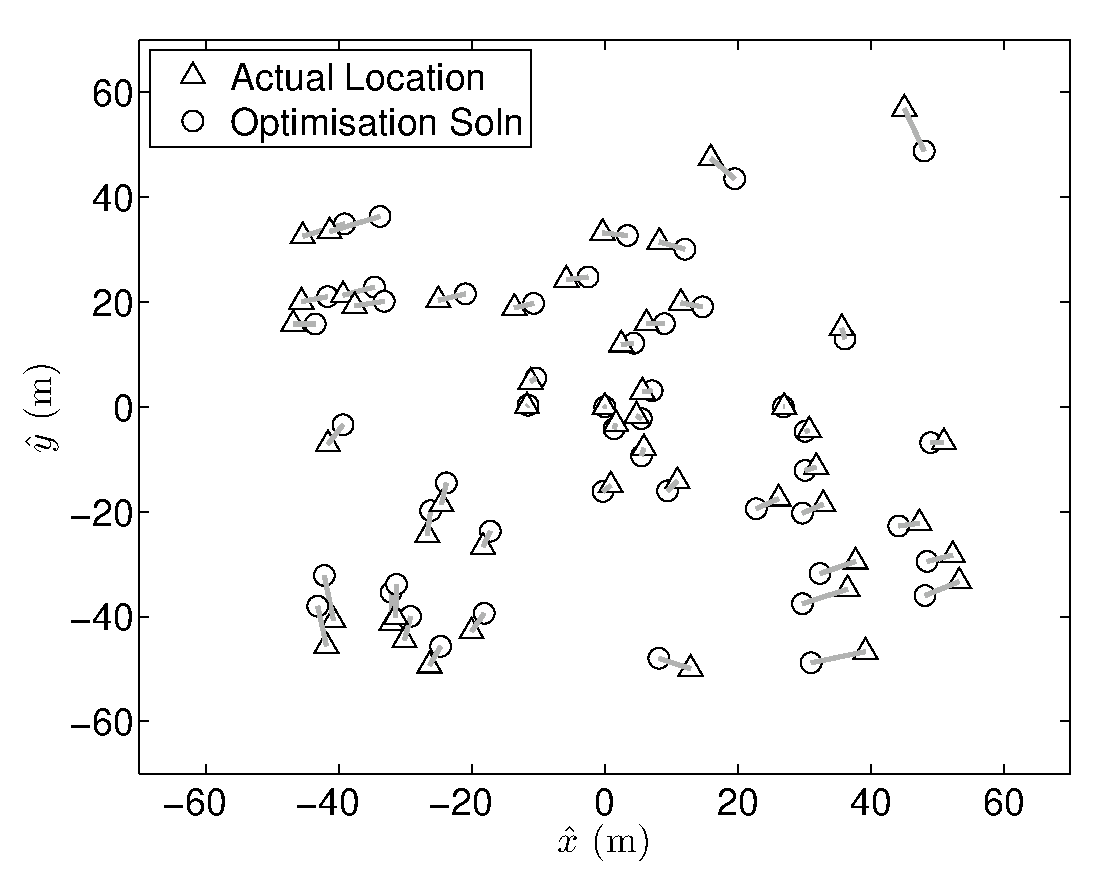
\includegraphics[width = 20pc]{diags/locs_2D_50eq_1.eps}
\caption{Example 1 - Synthetic relocation of 50 earthquakes in 2D
using all constraints with noise $\bar{\sigma}_N=0.02$. Actual and
optimization event locations are shown in triangles and circles,
respectively.} \label{fig-2D50eq-relocation_eg1}
\end{figure}

\begin{figure}
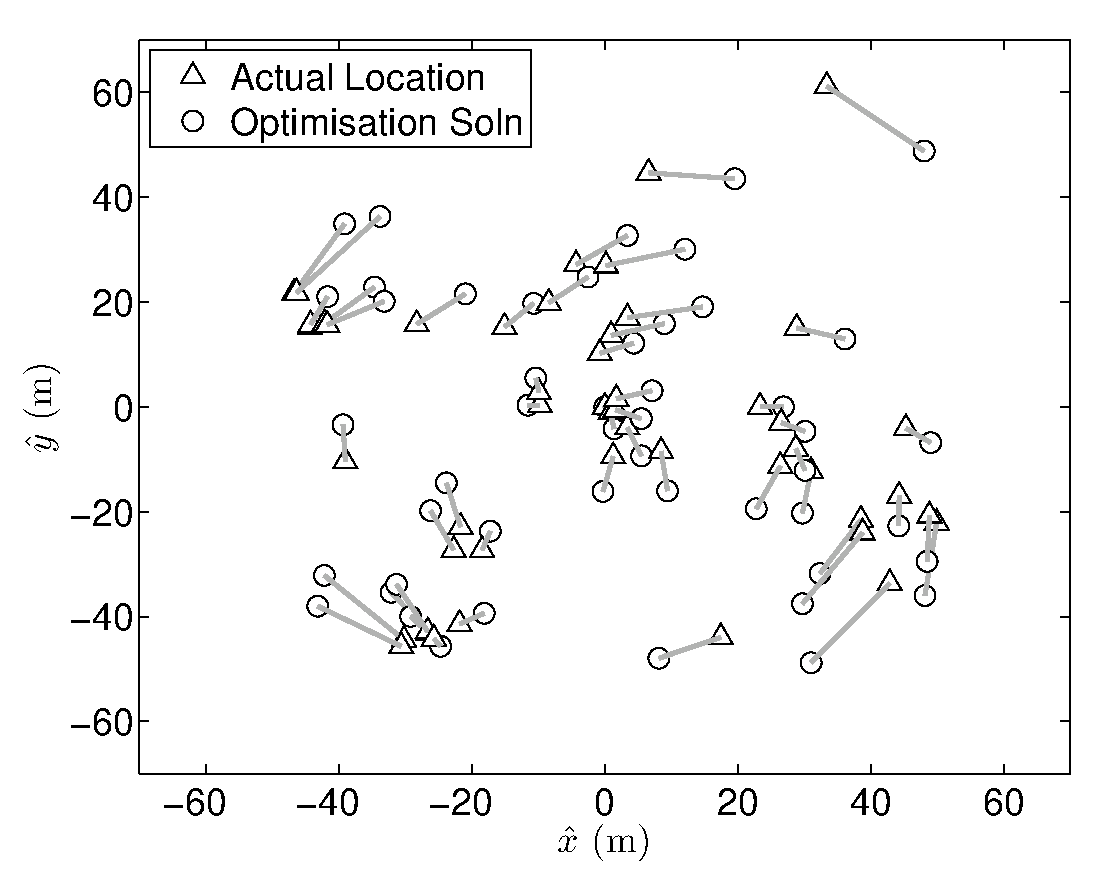
\includegraphics[width = 20pc]{diags/locs_2D_50eq_3.eps}
\caption{Example 2 - Synthetic relocation of 50 earthquakes in 2D
using all constraints with noise $\bar{\sigma}_N= 2
\sigma_{1to5Hz}(\delta_t)$.
 Actual and optimization event locations
are shown in triangles and circles, respectively.}
\label{fig-2D50eq-relocation_eg3}
\end{figure}
\citet{dr_Robinson11a} demonstrates that the noise on CWI estimates
is often larger than 0.02 and that it increases with event
separation. Consequently, example 1 is simplistic because we fix
$\bar{\sigma}_N=0.02$ for all pairs. In example 2 we increase the
uncertainty and introduce a distance dependance into the
hypothetical $\bar{\sigma}_N$ by defining
$\bar{\sigma}_N=\sigma_{1to5Hz}(\delta_t)$, where
$\sigma_{1to5Hz}(\delta_t)$ is the half-width of the errorbars for a
synthetic acoustic experiment with filtering between 1 and 5\,Hz
\citep[see Fig. 4(b) of ][]{dr_Robinson11a}. Repeating the
optimization leads to the circles in Figure
\ref{fig-2D50eq-relocation_eg3} which have an average coordinate
error of 2.8\,m.

Conjugate gradient based optimization techniques are susceptible to
the presence of local minima. This is because they use the slope of
the target function to explore the solution space. We explore the
impact of local minima for our CWI location problem by beginning the
optimization from 25 randomly chosen starting positions. We observe
no differences in the solution for either example.

Three observations can be drawn from the error structure in Figures
\ref{fig-2D50eq-relocation_eg1} and \ref{fig-2D50eq-relocation_eg3}.
Firstly, the location errors depicted by gray bars increase between
examples 1 and 2 with the introduction of larger noise. Secondly,
the errors are larger for events at greater distances from the
center. This is because events near the center of the cluster are
constrained by links from all angles, whereas those on the outside
are moderated by links from a limited number of directions. This
observation is analogous to problems associated with poor azimuthal
coverage in common triangulation problems such as individual
earthquake location from limited travel time data, or GPS
positioning with few satellites. Our third observation is that the
location errors are circular, despite our attempt to correct for
rotational non-uniqueness with the local coordinate system.

The local coordinate system works by constraining the location of
the first three earthquakes. Earthquake 1 is fixed at the origin,
earthquake 2 on the positive $\hat{x}$-axis and earthquake 3 has
$\hat{y}>0$. As the number of events increase the strength of these
constraints on later events weakens allowing small rotations of
events with respect to each other. That is, even though the
rotational freedom of the cluster is in principal removed by the
constraints imposed on the events (see equations
(\ref{eq:coord-const1}) to (\ref{eq:coord-const3})\footnote{equation
\ref{eq:coord-const4} is needed in 3D only}) we observe that in
practice the presence of noise allows the rotational non-uniqueness
to reappear. This is because the `easiest' way data noise can
propagate is into the direction which is least constrained by the
data. The same phenomena is observed in linear inversion where noise
creates large spurious model changes in directions of the
eigenvectors with the smallest singular values \citep{dr_Aster05a}.
Unfortunately, there is no obvious way to overcome this issue when
using coda waves alone since the constraints are based on
separation. Fortunately however, combining coda waves with
measurements of travel times alleviates this problem and facilitate
the removal of a local coordinate system altogether (see Section
\ref{sec:CalaverasLoc-CWIandTT}).

Despite our observations about the error structure however, we gain
confidence in the optimization procedure due to its stability for
different starting locations and because of the small average
coordinate errors of 2.0\,m and 2.8\,m for examples 1 and 2,
respectively.

\subsection{Example 3 - The impact of reduced linkage}

Synthetic examples 1 and 2 use 100\% direct linkage between event
pairs. That is, there is a constraint between each earthquake and
all other events. In reality, we might expect that the separation
between some pairs will not be constrained by CWI data due to poor
signal to noise ratio in the coda for common stations. Obviously,
the fewer stations that record an event the more likely it is that
links between it and other events will be broken. In such cases the
probabilistic distance constraint between a pair of events may only
exist indirectly through multiple pairs. In this section we consider
the impact of reduced linkage between event pairs. In example 3, we
repeat example 2 using 90\%, 80\%, ..., 10\% of the links. As with
the above examples, we undertake the optimization with 25 randomly
chosen starting locations.

\begin{figure}
%\noindent\includegraphics[width = 20pc]{../../thesis_version2/diags/eq_location_optimisation/synth2Dmulti/ressummary_2Dsynth50eq.eps}
\noindent\includegraphics[width =
20pc]{diags/synth2Dmulti/ressummary_2Dsynth50eq.eps}
\caption{Example 3 - Statistical measures of error in the
optimization solutions for the 2D synthetic cases when all (gray)
and best (black) results are considered. The statistics
$\Delta_{max}$ and $\Delta_\mu$  are the maximum and mean coordinate
error, respectively. The bottom subplot shows the average minimum
number of branches required to link the 2450 pairs.}
 \label{fig:optimisationresults-2Dsynth}
\end{figure}

Figures \ref{fig:optimisationresults-2Dsynth}(a) and (b) illustrates
the maximum $\Delta_{max}$ (top) and mean $\Delta_\mu$ (middle) of
the coordinate error as a function of increasing linkage. We show
the statistics for the `best' optimization solution (black) and for
the solution space when all 25 optimizations are considered (gray).
In the latter case the best solution is determined by the set of
event locations which lead to the smallest value of $L$. The error
in the best solution is consistent when 30\% or more of the branches
are used. The errors increase when only 10\% or 20\% of the
constraints are included. Interestingly, this breakdown around 20\%
to 30\% coincides with the point where the average number of
branches required to link each pair reaches 2 (see
Fig.\ref{fig:optimisationresults-2Dsynth} (bottom)). Since the
average number of branches can be computed in advance it can be used
as an indication of the inversion stability prior to optimization. A
higher breakdown is observed when all 25 solutions are considered
collectively. For example, the maximum coordinate error
$\Delta_{max}$ exceeds that for the best solution for linkage
$\leq$60\% confirming that the optimization is susceptible to local
minima and that a range of starting points should be considered.

Some optimizations fail to converge after 1200 iterations when the
linkage is 60\% or lower. All optimizations fail when then linkage
is 20\% or lower. Despite their failure to converge, the locations
at final iteration are close to the actual solution.

The derivatives used in the conjugate gradient method depend on
events connected by CWI measurements. Consequently, earthquakes that
are only connected via other events do not `communicate' with each
other directly. To some extent, this should be adressed during the
iterative process where location information can spread to events
which have no direct links. However, the lack of direct connection
through the gradient could prevent convergence in extreme cases, or
more likely slow the procedure down. This could explain why some
examples do not converge after 1200 iterations.
\citet{dr_VanDecar94a} show that gradient damping acts slowly
through iterative least-squares, because
 every cell in one iteration communicates only with its neighbours, and they demonstrate that this can be
fixed with preconditioning in some cases. Their findings suggest
that it may be possible to improve the convergence (stability and/or
speed) of the CWI optimization by preconditioning.

\subsection{Example 4 - 3D synthetic examples with reduced linkage}

In Example 4 we expand the optimization routine to 3D by randomly
picking
 a set of actual event locations for 50 earthquakes with
$-50$\,m$\leq \hat{x},\hat{y},\hat{z} \leq 50$\,m. As in the 2D case we assume a local velocity
of $v=3300\,$ms$^{-1}$ between all event pairs and a dominant frequency of 2.5$\,$Hz to represent
 waveform data filtered between 1 and 5$\,$Hz.
The hypothetical CWI mean is created using equation
(\ref{eq:hypothetical-CWI-mean-optichapt}) which ensures consistency
between the sample mean of hypothetical separation estimates and CWI
biases. We use a standard deviation for the noisy CWI estimates of
$\bar{\sigma}_N = \sigma_{1to5Hz}$ and perform the optimization
using 10\%, 20\%, ..., 100\% of the direct links. In each case we
repeat the optimization 25 times using randomly chosen starting
locations. The results are summarised in Figure
\ref{fig:optimisationresults-3Dsynth}.

\begin{figure}
%\noindent\includegraphics[width = 20pc]{../../thesis_version2/diags/eq_location_optimisation/synth3Dmulti/ressummary_3Dsynth50eq.eps}
\noindent\includegraphics[width =
20pc]{diags/synth3Dmulti/ressummary_3Dsynth50eq.eps}
\caption{Example 4 - Statistical measures of error in the
optimization solutions for the 3D synthetic cases when all (gray)
and best (black) results are considered. The statistics
$\Delta_{max}$ and $\Delta_\mu$ are the maximum and mean coordinate
error, respectively. The absence of the gray and black lines below
60\% and 30\% indicates a breakdown in the solutions when all or
best optimization result(s) are considered, respectively.}
\label{fig:optimisationresults-3Dsynth}
\end{figure}

When 70\% of the direct constraints are considered all optimization
results (gray) are consistent with the best solution (black). The
best solution constrains the event locations down to 30\% of the
direct links.

There is one notable difference between the 3D and 2D results. In 2D
the final iteration was close to the actual solution when the
optimization failed to converge. Conversely, in 3D the optimization
appears to converge to the correct solution or fail completely,
leading to a set of locations at final iteration which do not
resemble the actual solution. This is depicted in Figure
\ref{fig:optimisationresults-3Dsynth} by the absence of the gray and
black lines below 60\% and 30\% of the constraints, respectively.
The reason for this difference may be due to the increased number of
degrees of freedom in 3D requiring a greater number of iterations to
converge. Nevertheless, the accurate convergence of the best
solution for cases with 30\% linkage or higher is encouraging for
the potential of coda wave optimization to constrain earthquake
location.

\subsubsection{Summary of synthetic experiments}

In summary, the synthetic examples demonstrate the ability of coda
wave data to constrain relative event location using optimization.
The optimization error is influenced by the noise on CWI estimates
with greater $\bar{\sigma}_N$ leading to larger errors in the
solutions. When 70\% or more of the direct branches are used the
optimiser is stable with no observable difference in the solution
for 25 randomly chosen starting locations. As the direct linkage
reduces to 50\% the optimization becomes less stable and the best
solution from 25 random starting locations is required to find the
optimal solution. As the number of links decrease below 30\% the
best solution fails to converge.


\section{Relocating Earthquakes on the Calaveras Fault}
\label{sec:CalaverasLoc-CWIonly}

In this section we relocate 68 earthquakes from the Calaveras Fault,
California. The 68 earthquakes are selected from the 308 earthquake
Calaveras example released with the open source Double Difference
algorithm or hypoDD \citep{dr_Waldhauser00a, dr_Waldhauser01a}[See
also Data and Resources Section]. These events are chosen for three
reasons. Firstly, they are recorded by a large number of stations
(Fig. \ref{fig:-eqopti-California-Calaveras}) and therefore lend
themselves to accurate travel time location. This makes them ideal
for assessing the performance of a new location technique. Secondly,
they are distributed with separations from near zero to hundreds
meters making them ideal for application of CWI. Finally, Calaveras
earthquakes have been well researched with several studies having
relocated events in the region \citep{dr_Waldhauser01a,
dr_Schaff02a, dr_Waldhauser08a}. The relocations in this paper are
sorted into four examples summarised in Table \ref{tab:examples}.


\begin{figure}
\noindent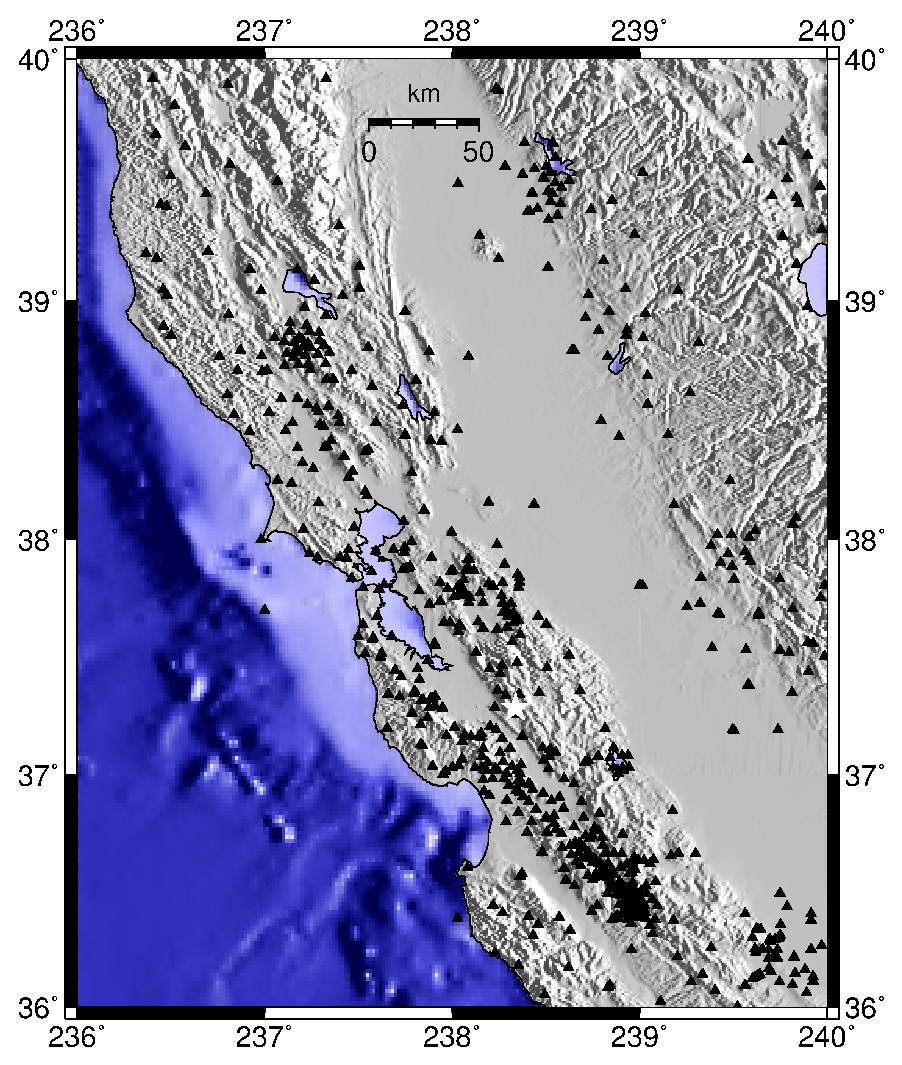
\includegraphics[width =
20pc]{diags/CalaverasMap/gmt_california/CaliforniaCalaverasMap1.eps}
\caption{Elevation in California showing location of the Calaveras
cluster (white star) and 805 seismic stations (black triangles).}
\label{fig:-eqopti-California-Calaveras}
\end{figure}


\begin{table}
\caption{Location examples for the 68 Calaveras earthquakes.}
\label{tab:examples}
\begin{tabular}{ll}
\hline
Example 5 & Comparison of CWI, catalogue and hypoDD \\
 & locations (using all available data). \\
Example 6 & Exploration of station dependance for CWI and \\
 & hypoDD (using a subset of data). \\
Example 7 & Combined use of CWI and travel time data \\
& with all and a reduced number of stations. \\
Example 8 & Combined use of CWI and travel time data \\
 & when travel times constrain only 50\% of the events. \\
 \hline
\end{tabular}
\end{table}



\subsection{Example 5 - comparison of CWI, catalogue and hypoDD locations}

Figure \ref{fig-69Calaverasevents_eg1} illustrates three sets of
locations for the Calaveras earthquakes. The first column shows the
original catalogue locations for all 308 earthquakes. That is, each event
is located individually using all available travel time arrivals and
a regional velocity model. The 68 earthquakes of interest in this
study are differentiated in black. Catalogue locations suggest that
the 68 earthquakes of interest are distributed spatially throughout
all events.

%%=======================================================================================
% This is the original figure using HypoDD with LSQR
%\begin{figure*}
%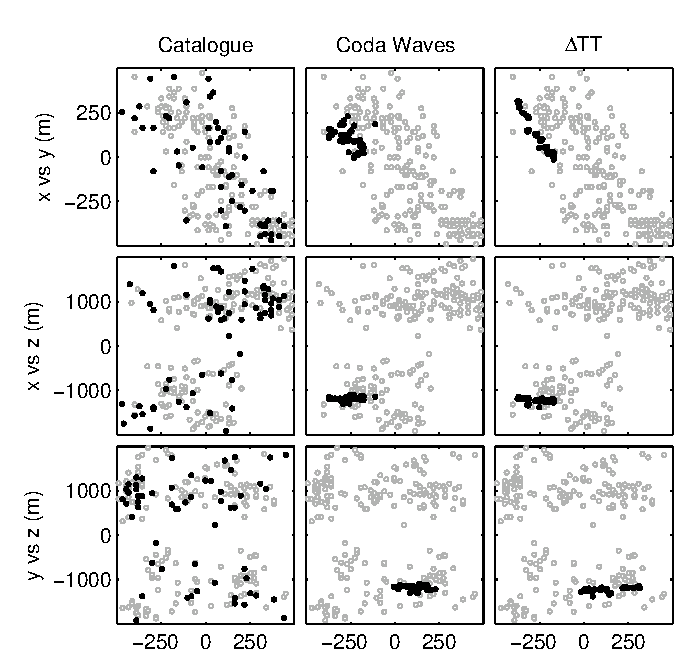
\includegraphics{diags/CalaverasLoc1.eps}
%\caption{Comparison of earthquake hypocenters using three different methods: catalogue location (column 1), hypoDD with all
%308 events (column 2) and CWI example 1 (column 3).
%Note that in the case of the CWI locations we consider only the 68 earthquakes in red, the
%blue events are shown for the purpose of orientation only.}
%\label{fig-69Calaverasevents_eg1}
%\end{figure*}

% Now we have the SVD version
\begin{figure*}
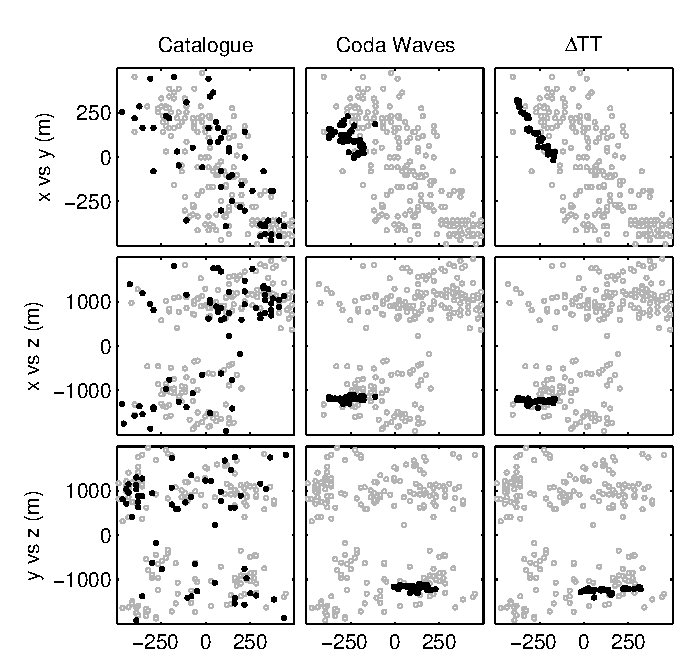
\includegraphics{diags/CalaverasLoc1_hypoDD_SVD.eps}
\caption{Example 5 - Comparison of relative earthquake locations
using three different methods: catalogue location (column 1), CWI
(column 2) and hypoDD (column 3). Note that in the case of the
hypoDD and CWI inversions we consider only the 68 earthquakes in
black, the gray catalogue locations for the remaining 240 (308-68)
earthquakes are shown for the purpose of orientation only.}
\label{fig-69Calaverasevents_eg1}
\end{figure*}
%%=======================================================================================

To apply CWI we download available waveforms from the Northern
California Earthquake Data Center (See Data and Resources Section).
Unsuitable waveforms are removed using the conditions summarised in
Table 5 of \citet{dr_Robinson11a}. Remaining waveforms are filtered
between 1 and 5\,Hz and aligned  to $P$ arrivals at 0\,s. CWI
estimates are obtained from 5\,s wide non-overlapping time windows
between $2.5 \leq t \leq 20$\,s and used to create probabilistic
constraints on event separation. We introduce the local coordinate
system of Section \ref{sec:theory} and find the optimum relative
locations using Polak-Ribiere optimization.

CWI locations for the 68 events are illustrated in column two of
Figure \ref{fig-69Calaverasevents_eg1}. Catalogue locations (gray)
are shown for the remaining 240 earthquakes and are included to ease
comparison. The third column of Figure
\ref{fig-69Calaverasevents_eg1} illustrates the locations given by
hypoDD with Singular Value Decomposition (SVD), absolute arrival
times and cross correlation computed travel time differences.

Global locations cannot be found by CWI alone. For the sake of
comparison, we arbitrarily choose a `master' event and translate our
relative locations to align with the hypoDD location for the same
event. This arbitrary translation does not change the relative
locations. We return to this issue of relative versus actual
location in Example 7 by introducing a combined travel time and coda
wave inversion.

The spatial distribution of the CWI locations is clearly tighter
than the catalogue locations of column 1. That is, CWI provides an
independent indication of clustering for the 68 events and to first
order, similar locations to those from hypoDD (column 3). There is a
small second order difference between the CWI and hypoDD based
locations. In particular, the lineation is less clear in the CWI
locations (column 2) than the hypoDD locations (column 3). Our
results suggest that the coda are less supportive of the presence of
streaks although a complete understanding of these differences is
left for future work. Our attention now is devoted towards
understanding how both techniques perform with fewer stations
(Example 6) and exploring how CWI and travel times can be combined
(Examples 7 and 8).


\subsection{Example 6 - Dependance on the number of stations}


Accurate location of the Calaveras events is possible using arrival
phases because of the excellent recording situation in California
with many stations and strong azimuthal coverage (see Fig.
\ref{fig:-eqopti-California-Calaveras}). In contrast, a small number
of stations and poor azimuthal coverage are common limitations when
trying to locate intraplate clusters. For example, there are only
four network seismic stations in the South West Seismic Zone of
Western Australia, a region similar in size to that hosting 805
stations in Figure \ref{fig:-eqopti-California-Calaveras}.

We explore the impact of poorer recording situations in example 6 by
re-locating the 68 Calaveras events  using hypoDD and coda waves
with a reduced number of stations. We begin with 10 stations and
repeat the process removing one at a time until a single station
remains. The 10 stations considered are shown in Figure
\ref{fig:-eqopti-Calaveras-substations} and the order of removal
explained in Table \ref{tab:Calaveras-stationremoval}.


\begin{figure}
\noindent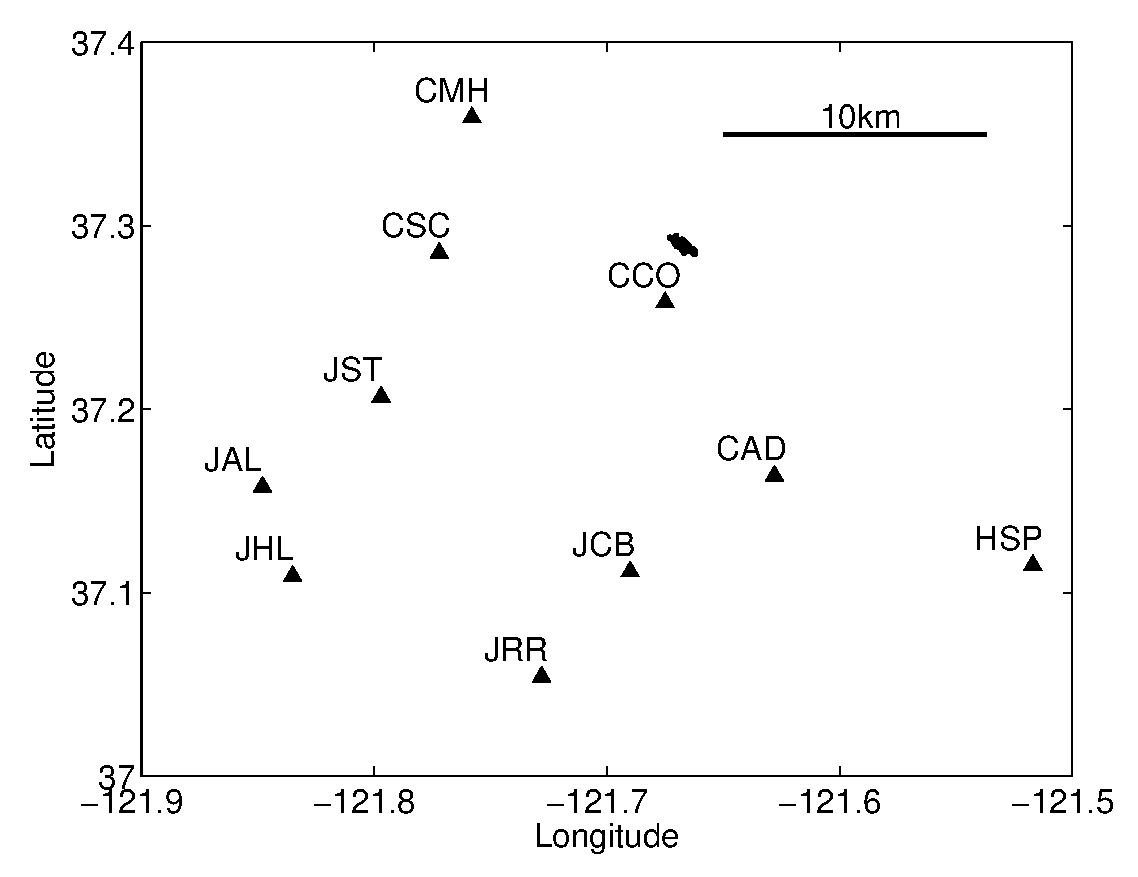
\includegraphics[width =
20pc]{diags/CalaverasMap/matlab/Calaveras_substationmap}
\caption{Location of the 10 stations (triangles) used to relocate
the Calaveras events in Example 6 to 8. Stations are removed one at
a time according to the order in Table
\ref{tab:Calaveras-stationremoval} and the events relocated. The
events are indicated with black circles.}
\label{fig:-eqopti-Calaveras-substations}
\end{figure}

\begin{table}
\caption{Stations considered when exploring the impact of reduced
station coverage.} \label{tab:Calaveras-stationremoval}
\begin{tabular}{|r|l|}
\hline
Number of & Station Names\\
Stations  & \\
\hline
10 & CCO, JCB, JST, CMH, HSP, JAL, CSC, JST, CAD, JHL, JRR\\
9  & CCO, JCB, JST, CMH, HSP, JAL, CSC, JST, CAD, JHL\\
8  & CCO, JCB, JST, CMH, HSP, JAL, CSC, JST, CAD\\
7  & CCO, JCB, JST, CMH, HSP, JAL, CSC \\
6  & CCO, JCB, JST, CMH, HSP, JAL \\
5  & CCO, JCB, JST, CMH, HSP \\
4  & CCO, JCB, JST, CMH \\
3  & CCO, JCB, JST \\
2  & CCO, JCB \\
1  & CCO \\
\hline
\end{tabular}
\end{table}


CWI locations are illustrated in Figure
\ref{fig-CWIreducesstats} for the inversions with 7, 5, 4, 3, 2 and
1 station. We observe a high level of consistency between these 6
inversions and the locations shown in Figure
\ref{fig-69Calaverasevents_eg1} (column 2) when all stations are
considered. That is, the coda wave approach is self-consistent
regardless of the number of stations available, reinforcing our
hypothesis that coda waves can constrain location in poor recording
situations.

\begin{figure*}
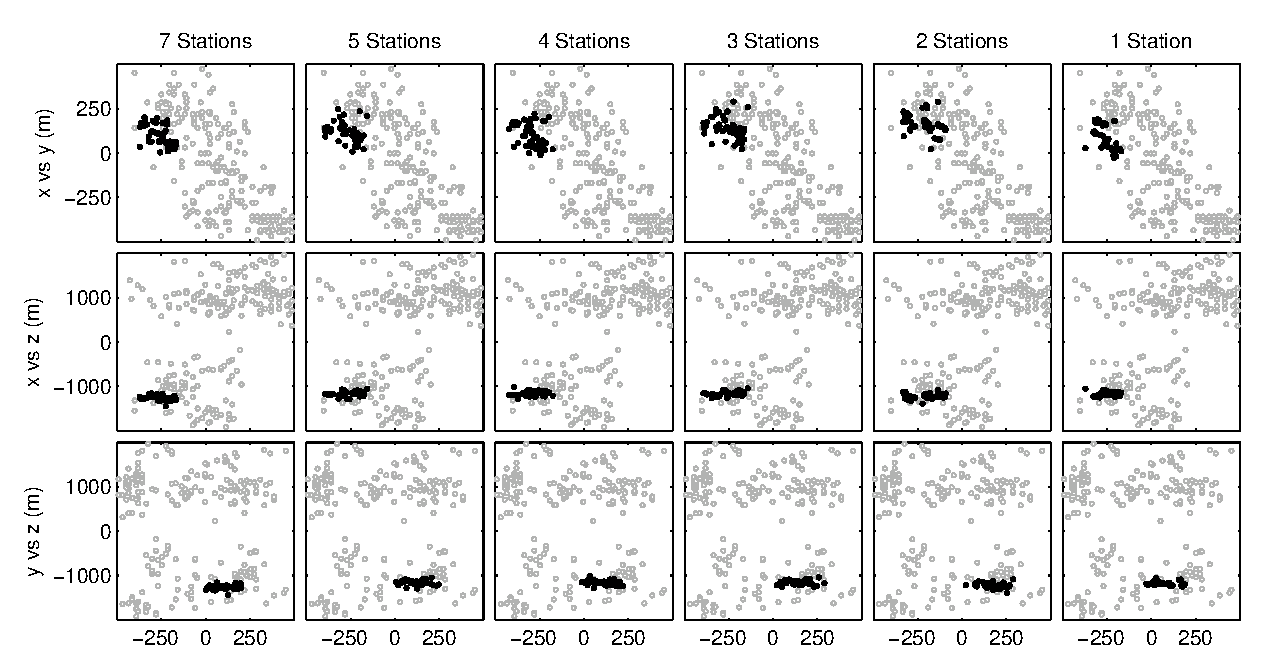
\includegraphics[angle=90,height = 50pc]{diags/CalaverasLoc2.eps}
\caption{Example 6 - CWI relative locations with reduced stations.}
\label{fig-CWIreducesstats}
\end{figure*}


Figure \ref{fig-HYPODDreducesstats} illustrates the hypoDD inversion
results for seven, five and four stations. The travel time problem
is ill-posed for fewer than four stations so it is not possible to
apply hypoDD with SVD for three or fewer stations.  The hypoDD
locations are not self-consistent as the number of stations is
reduced. We observe a general increase in scatter and a higher
number of stray events outside the cluster when less stations are
used with hypoDD. Even with seven stations the linear geometry of
Figure \ref{fig-69Calaverasevents_eg1} (column 3) is less evident.

%%=========================================================================
% this is the original version using hypoDD with LSQ
%\begin{figure*}
%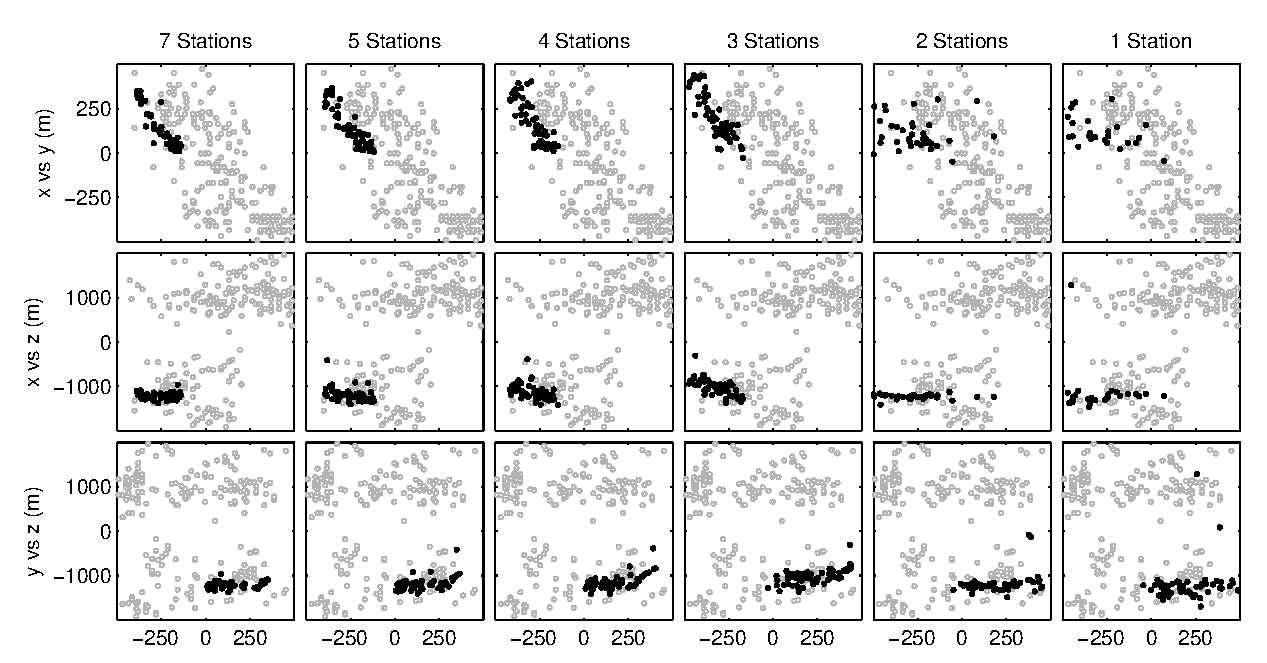
\includegraphics[angle=90,height = 50pc]{diags/CalaverasLoc3.eps}
%\caption{....}
%\label{fig-HYPODDreducesstats}
%\end{figure*}

% This is the version using hypoDD with SVD
\begin{figure*}
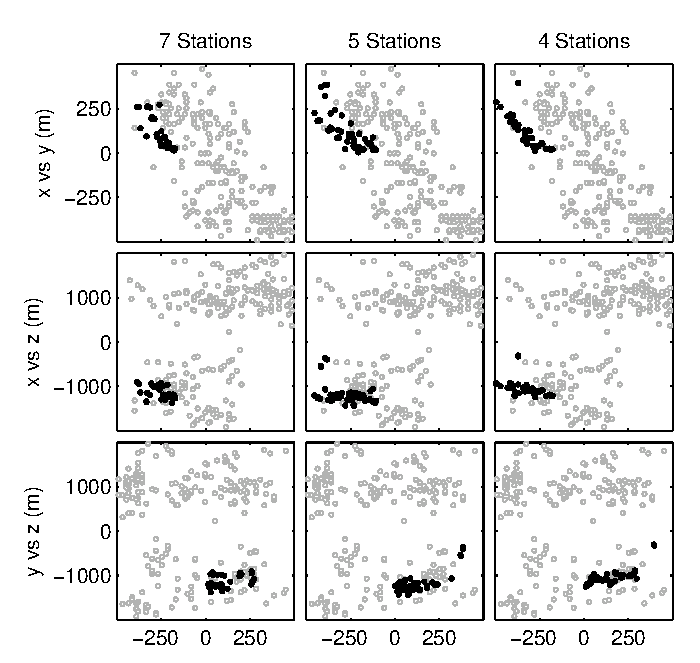
\includegraphics[height = 25pc]{diags/CalaverasLoc3_hypoDD_SVD.eps}
\caption{Example 6 - HypoDD (SVD) relative locations with reduced
stations.} \label{fig-HYPODDreducesstats}
\end{figure*}
%%=========================================================================


As the number of stations are reduced both the CWI and hypoDD
techniques are not able to re-locate all events. To use the coda
waves we need at least one pairwise separation constraint to be
formed from the available stations. This means that for every event
there must be at least one station that records it and at least one
other earthquake sufficiently well to apply CWI. Fortunately, we can
make an assessment of this prior to starting the inversion. The top
row of Figure \ref{fig-statremoval_summarystats} demonstrates that
when five or more stations are used, CWI can constrain the location
of all 68 earthquakes. When less than five stations are used the
coda waves constrain a decreasing number of events until at one
station it is only possible to locate 55 of the 68 events.

%%=========================================================================
% This is the original version using hypoDD with LSQ
%\begin{figure}
%\noindent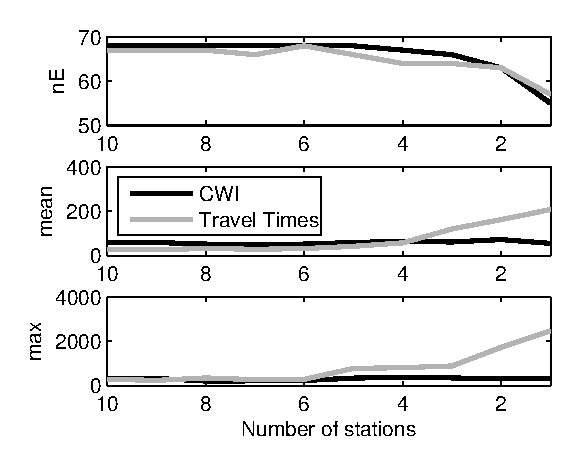
\includegraphics[width = 20pc]{diags/CalaverasLoc4.eps}
%\caption{Statistics on coordinate differences for reduced station inversions. Differences
%are computed between the inversion results (CWI and hypoDD) and the complete hypoDD
%locations for all 308 events. The top subplot illustrates the number of constrainable
%events in the CWI and hypoDD inversions as a function of the stations considered.}
%\label{fig-statremoval_summarystats}
%\end{figure}

% This is the version using hypoDD with SVD
\begin{figure}
\noindent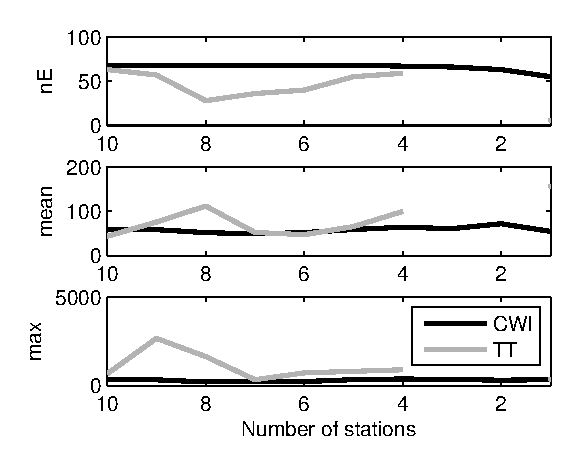
\includegraphics[width =
20pc]{diags/CalaverasLoc4_hypoDD_SVD.eps} \caption{Example 6 -
Statistics on coordinate differences for reduced station inversions.
Differences are computed between the inversion results (CWI and
hypoDD) and the complete hypoDD locations for all 308 events. The
top subplot illustrates the number of constrainable events,$nE$ in
the CWI and hypoDD inversions as a function of the stations
considered.} \label{fig-statremoval_summarystats}
\end{figure}
%%=========================================================================


The hypoDD program also struggles to locate all events as the number
of stations is reduced. In the case of hypoDD an event can be
identified as unconstrainable in one of two stages. Firstly, the
data are analysed to ensure that there exists travel time
differences for each event and at least one other earthquake. This
is analogous to the situation for the coda wave technique. The
hypoDD program also has a secondary identification phase in which
events that can not be located sufficiently are rejected during the
inversion. This process is presumably related to the iterative
removal of outliers described by \citet{dr_Waldhauser00a}. The top
row of Figure \ref{fig-statremoval_summarystats} shows that the
number of events re-located by hypoDD fluctuates between 63 and 28
earthquakes for 10 to 4 stations and it demonstrates that the number
of events located by hypoDD is less than the number located by CWI
in all cases.

The remaining rows of Figure \ref{fig-statremoval_summarystats}
illustrate a statistical comparison of the CWI and hypoDD reduced
station locations to those using hypoDD with all available data. For
the CWI inversions the mean and maximum coordinate difference is
consistent regardless of the number of stations considered. In
contrast, the hypoDD mean and maximum coordinate error fluctuate
above those for CWI confirming that the hypoDD inversion is less
stable than CWI with fewer stations.

\section{Theory for Combining travel time and CWI constraints}
\label{sec:CalaverasLoc-CWIandTT}
In Examples 5 and 6 we compare the location of the Calaveras
earthquakes using coda wave and arrival time based constraints
independently. Since the arrival time (direct or difference) and
coda wave data
 come from different sections of the waveform they provide independent constraints on the locations.
 In this section we devise a location algorithm which incorporates
 both CWI and travel time data.

We do not propose a new technique for earthquake location using
travel time differences. Rather, we exploit the information created
by hypoDD with SVD to define a probability density (or posterior)
function
\begin{equation}
\label{eq-multi-var-Gauss-tt}
\begin{array}{l}
P(\mathbf{e}_p|\Delta_{TT})
\frac{1}{(2\pi)^{\frac{3}{2}}\sqrt{|\Sigma|}} \\
\hspace{5em} \times \exp
\left({-\frac{1}{2}\left([\mathbf{e}_p-\mu_{\mathbf{e}_p}]^T
\Sigma^{-1} [\mathbf{e}_p-\mu_{\mathbf{e}_p}]\right)} \right),
\end{array}
\end{equation}
where
\begin{equation}
\mathbf{e}_p = (x_p,y_p,z_p)^T
\end{equation}
is the location of event $p$,
\begin{equation}
\mu_{\mathbf{e}_p} = (\mu_{x_p}, \mu_{y_p},\mu_{z_p})^T
\end{equation}
is the most likely location as determined using the travel time
data, and
\begin{equation}
\label{eq:Sigma-expression}
\Sigma = \left( \begin{array}{ccc} \sigma_{x_p}^2 & 0 & 0\\
0 &  \sigma_{y_p}^2 & 0 \\
0 & 0 & \sigma_{z_p}^2  \end{array} \right)
\end{equation}
is the covariance matrix. In this paper we define the mean location
$\mu_{\mathbf{e}_p}$ and covariance matrix by the hypoDD optimum
solution and its uncertainties. It is important to note that hypoDD
must be used with SVD to obtain useful estimates of $\sigma_{x_p}$,
$\sigma_{y_p}$ and $\sigma_{z_p}$ because the errors reported by
conjugate gradient methods (LSQR) are grossly underestimated in
hypoDD \citep{dr_Waldhauser01a}.

We pose the location problem using the negative log likelihood
\begin{equation}
\label{eq-Lstar-tt-cwi}
\begin{array}{l}
 L(\mathbf{e}_1, \mathbf{e}_2, ...,
\mathbf{e}_1, \mathbf{e}_n) = - \sum_{i=1}^n
ln\left[P(\mathbf{e}_i|\Delta_{TT})\right] \\
\hspace{6em}  - \sum_{i=1}^{n-1}
\sum_{j=i+1}^n
ln\left[P(\delta_{CWIN}|\mathbf{e}_i,\mathbf{e}_j)\right],
\end{array}
\end{equation}
where $(\mathbf{e}_1, \mathbf{e}_2, ..., \mathbf{e}_n)$ is the joint
location,
\begin{equation}
\label{eq-ttcomponent} \sum_{i=1}^n
ln\left[P(\mathbf{e}_i|\Delta_{TT})\right]
\end{equation}
incorporates the travel time constraints and
\begin{equation}
\label{eq-codacomponent} \sum_{i=1}^{n-1} \sum_{j=i+1}^n
ln\left[P(\delta_{CWIN}|\mathbf{e}_i,\mathbf{e}_j)\right]
\end{equation}
 the coda waves.

We must differentiate $L$ to use the Polak-Ribiere conjugate
gradient technique of \citet{dr_Press87a}. The derivative of
$L(\mathbf{e}_1, \mathbf{e}_2, ..., \mathbf{e}_n)$ with respect to
$x_p$ is given by
\begin{equation}
\begin{array}{l}
\frac{\partial L}{\partial x_p} =  - \frac{\partial ln\left[P(\mathbf{e}_p|t_{DD})\right]}{\partial x_p}
- \sum_{i=p+1}^{N} \frac{ \partial \ln
\left[P(\delta_{CWIN}|\mathbf{e}_p,\mathbf{e}_i)\right]}{\partial
x_p} \\
\hspace{5em} - \sum_{j=1}^{p-1} \frac{ \partial \ln
\left[P(\delta_{CWIN}|\mathbf{e}_j,\mathbf{e}_p)\right]}{\partial
x_p}
\end{array}
\end{equation}
where
\begin{equation}
\sum_{i=p+1}^{N} \frac{ \partial \ln
\left[P(\delta_{CWIN}|\mathbf{e}_p,\mathbf{e}_i)\right]}{\partial
x_p}
\end{equation}
and
\begin{equation}
\sum_{j=1}^{p-1} \frac{ \partial \ln
\left[P(\delta_{CWIN}|\mathbf{e}_j,\mathbf{e}_p)\right]}{\partial
x_p}
\end{equation}
are defined in Appendix \ref{sec-Appendix-derivatives_ofL} and
\begin{equation}
\begin{array}{l}
\frac{\partial ln\left[P(\mathbf{e}_p|t_{DD})\right]}{\partial x_p}
= -\frac{1}{2}[1,0,0]^T \Sigma^{-1}
[\mathbf{e}_p-\mu_{\mathbf{e}_p}] \\
\hspace{9em} -\frac{1}{2}
[\mathbf{e}_p-\mu_{\mathbf{e}_p}]^T \Sigma^{-1} [1,0,0].
\end{array}
\end{equation}
Similarly, for the derivatives with respect to $y_p$ and $z_p$ we
have
\begin{equation}
\begin{array}{l}
\frac{\partial ln\left[P(\mathbf{e}_p|t_{DD})\right]}{\partial y_p}
= -\frac{1}{2} [0,1,0]^T \Sigma^{-1}
[\mathbf{e}_p-\mu_{\mathbf{e}_p}] \\
\hspace{9em} -\frac{1}{2}
[\mathbf{e}_p-\mu_{\mathbf{e}_p}]^T \Sigma^{-1} [0,1,0]
\end{array}
\end{equation}
and
\begin{equation}
\begin{array}{l}
\frac{\partial ln\left[P(\mathbf{e}_p|t_{DD})\right]}{\partial z_p}
= -\frac{1}{2} [0,0,1]^T \Sigma^{-1}
[\mathbf{e}_p-\mu_{\mathbf{e}_p}] \\
\hspace{9em} -\frac{1}{2}
[\mathbf{e}_p-\mu_{\mathbf{e}_p}]^T \Sigma^{-1} [0,0,1].
\end{array}
\end{equation}

Combining the travel time and coda wave data offers two advantages.
Firstly, it combines independent constraints on the event locations
offering further confidence in the resulting solution. Secondly, the
travel time constraints in the form of equation
(\ref{eq-ttcomponent}) resolve the inherent non-uniqueness
associated with translation, rotation and reflection around a global
coordinate system. This means that it is no longer necessary to use
a local coordinate system and we can solve directly for location
with respect to a global reference. Collectively, these advantages
improve the behavior of the Polak-Ribiere optimization leading to
faster and more stable convergence. Consequently, we no longer have
to consider multiple randomly chosen starting locations.


\subsection{Example 7 - Combining travel time and CWI constraints}
 Figure
\ref{fig-68Calaverasevents_ttandcoda1} illustrates the earthquake
locations obtained when we combine the travel time and coda wave
data using all data (left) and five stations (right). The linear
features observed in the original hypoDD inversions (see Fig.
\ref{fig-69Calaverasevents_eg1}) are evident in both cases. However,
the coda waves introduce a scatter around these streaks. That is,
the locations in figure \ref{fig-68Calaverasevents_ttandcoda1}
result from a trade-off between hypoDD's desire to place the events
on linear features and the coda waves voracity to push them away
from streaks. When all stations are used the hypoDD constraints are
strong and little off-streak scatter is introduced. As we reduce
hypoDD's leverage by decreasing the number of stations to five, we
observe an increase in off-streak scatter resulting from the
enhanced influence of the coda.

%%=========================================================================
% This is the original version using hypoDD with LSQ
% This is only makes sense for LSQR so we remove it from this manuscript
%\begin{figure*}
%\noindent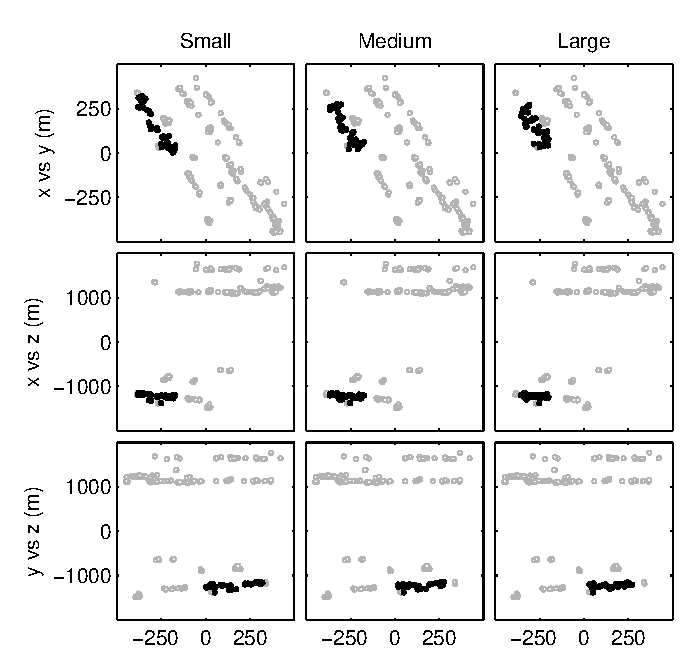
\includegraphics{diags/CalaverasLoc5.eps}
%\caption{Locations of the 68 Calaveras earthquakes combining all available coda wave and travel time constraints with three different
%levels of uncertainty on the travel time PDFs. Column 1 sets $\sigma_x = \sigma_y = 19.5$\,m and $\sigma_z = 15$\,m
%\citep[after]{dr_Waldhauser08a}, Column 2 uses $\sigma_x = \sigma_y = 3 \times19.5$\,m and $\sigma_z = 3\times15$\,m and
%column 3 considers $\sigma_x = \sigma_y = 152$\,m and $\sigma_z = 232$\,m \citep[after]{dr_Shearer97a}. }
%\label{fig-68Calaverasevents_ttandcoda1}
%\end{figure*}

% This is the version using hypoDD with SVD
\begin{figure}
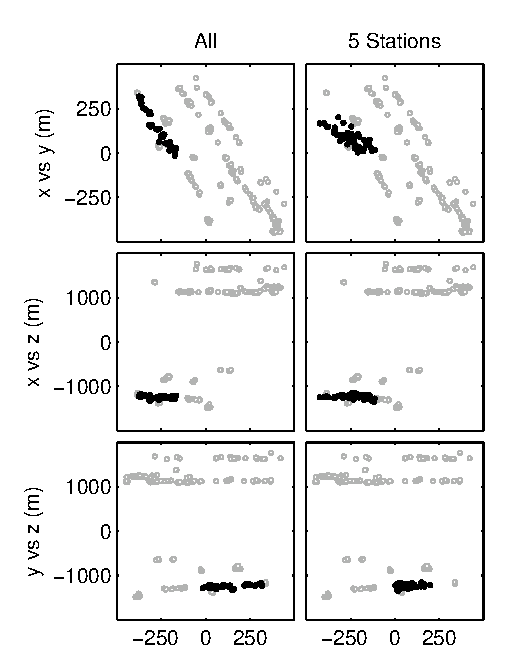
\includegraphics{diags/CalaverasLoc5_hypoDD_SVD.eps}
\caption{Example 7 - Combined HypoDD (SVD) and CWI relative
locations using data form all stations (left) and 5 stations
(right).} \label{fig-68Calaverasevents_ttandcoda1}
\end{figure}


%%=========================================================================


\subsection{Example 8 - Combining CWI and travel times when the travel times constrain a limited number of events}


In intraplate regions such as Australia it is common to deploy
temporary seismometers to monitor aftershocks for significant events
\citep{dr_Bowman90a, dr_Leonard02a}. Traditionally, these
deployments facilitate a higher accuracy of location for events
occuring during the deployment period. Using our combined inversion
it is possible to re-locate all events by employing the detailed
travel time data when the temporary network is in-situ and using
coda waves from network stations when the deployment is absent. The
hypothesis, to be tested in this section, is that conducting such a
combined inversion will improve the location accuracy of events
outside the deployment period.

An estimate of the cummulative number of aftershocks $N(t)$ after
$t$ days is given by the modified Omori formula
\begin{equation}
\label{eq:CumOmori}
 N(t) = K \frac{c^{1-p} + (t+c)^{1-p}}{p-1}
\end{equation}
\citep{dr_Utsu95a}.
The empirically derived constants, $K$, $C$ and $p$ vary between
tectonic settings. For example, using recorded aftershocks with
$M\ge3.2$ of the  Hokkaido-Nansei-Oki, Japan $M_s=7.8$ earthquake of
12 July 1993, \citet{dr_Utsu95a} obtained maximum likelihood
estimates for $K$, $p$ and $c$ of 906.5, 1.256 and 1.433,
respectively.  With these empirically derived values an array
deployed within 4 days and left for 150 days will record roughly one
half of the aftershocks occurring within the first 1000 days. That
is,
\begin{equation}
\frac{N(150+4)-N(4)}{N(1000)} = \frac{2257-934}{2626} \approx 0.5.
\end{equation}
This idea is illustrated in Figure \ref{fig:Omorifigure} which shows
the best fitting Omori Formula separated into segments before
(gray), during (black) and after (gray) the pseudo temporary
deployment.

\begin{figure}
\noindent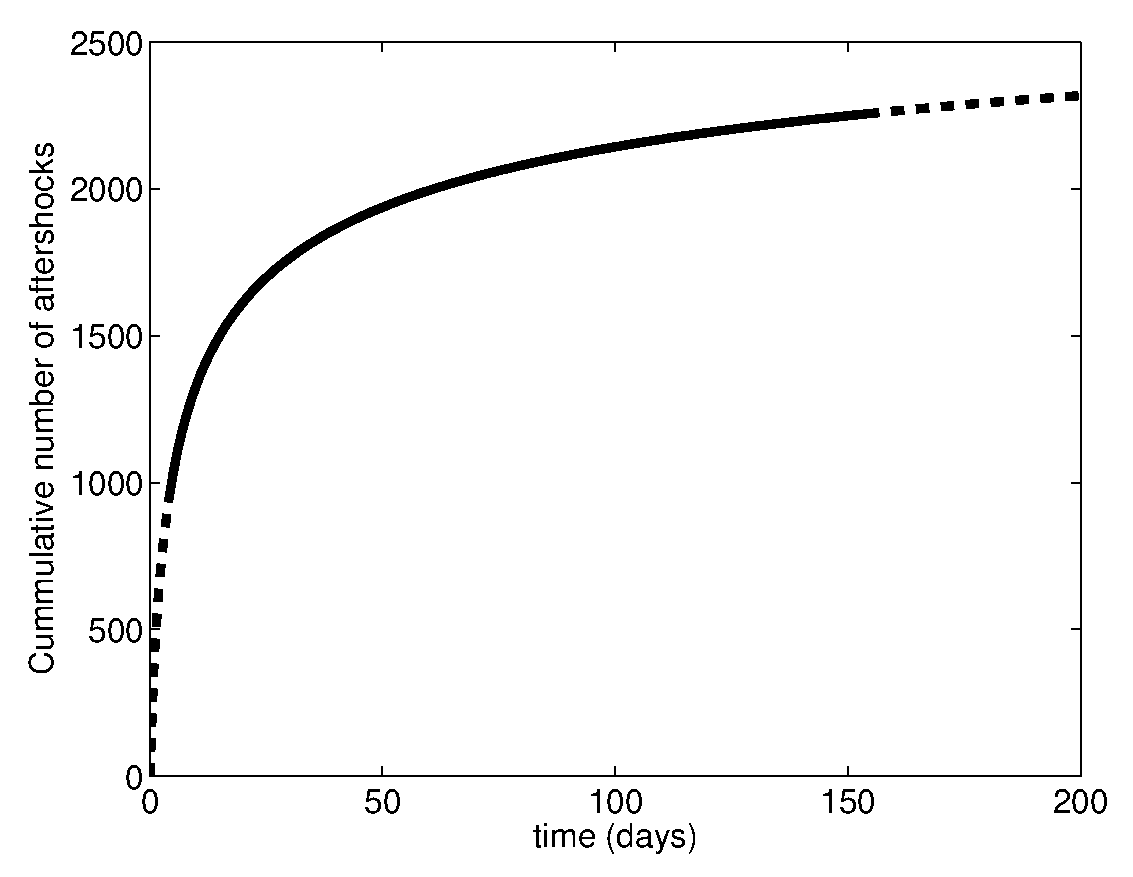
\includegraphics[width = 20pc]{diags/OmoriFigure.eps}
\caption{Cumulative number of aftershocks for the
Hokkaido-Nansei-Oki, Japan $M_s=7.8$ earthquake of 12 July 1993
using equation (\ref{eq:CumOmori}). The leftmost gray, middle black
and rightmost gray lines signify aftershocks occurring before,
during and after the deployment of a pseudo temporary array
installed 4 days after the main shock and left for 150 days. A
temporary deployment of this kind will record roughly 50\% of the
aftershocks in the 1000 days following the mainshock. }
\label{fig:Omorifigure}
\end{figure}

With this idea of a temporary deployment in mind we have another
attempt at relocating the Calaveras earthquakes. In Example 8 we
consider the travel time constraints on half (34) of the earthquakes
and incorporate coda wave data from a single station for all 68
earthquakes. The combined inversion is shown in column 1 of Figure
\ref{fig-68Calaverasevents_ttsubsetandcoda1}. The inversion result
is similar to the combined inversion when all travel time data is
incorporated (see Fig. \ref{fig-68Calaverasevents_ttandcoda1}). The
slight increase in scatter observed here can be explained by the
events with no travel time constraints and the tendency of the coda
to push events away from streaks.

Remarkably, the combined coda wave and travel time inversion locates
all 68 earthquakes to an accuracy similar to the inversions with all
data. In contrast when travel time data is used alone it is only
possible to locate the 34 events recorded by the pseudo temporary
deployment. This
ability of  coda waves to constrain the location of events recorded
by a single station creates new opportunities for understanding
earthquakes in regions with limited station coverage.

%%=========================================================================
% This is the original version using hypoDD with LSQ
%\begin{figure}
%\noindent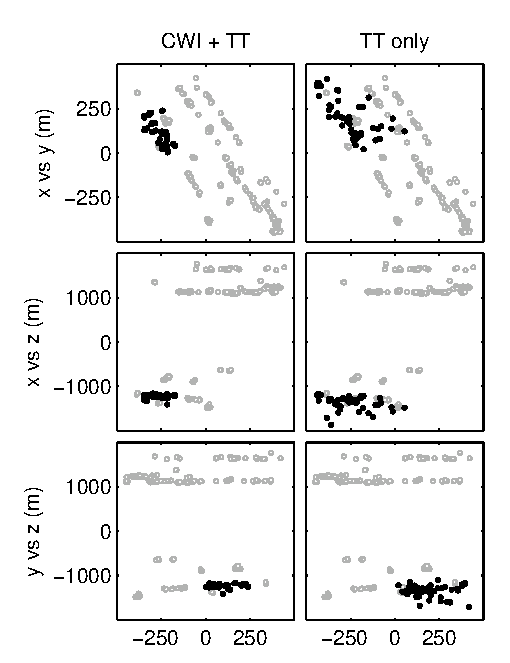
\includegraphics{diags/CalaverasLoc6.eps}
%\caption{Left - Combined travel time and coda wave inversions using travel time constraints on
%22 (or 32\%) of the events and coda waves from station CCO only. All travel time based uncertainties
%are assigned $\sigma_x = \sigma_y = 3 \times19.5$\,m and $\sigma_z = 3\times15$\,m. Right - travel time
%relocation only (i.e. no CWI) using ........}
%\label{fig-68Calaverasevents_ttsubsetandcoda1}
%\end{figure}

% This is the version using hypoDD with SVD
\begin{figure}
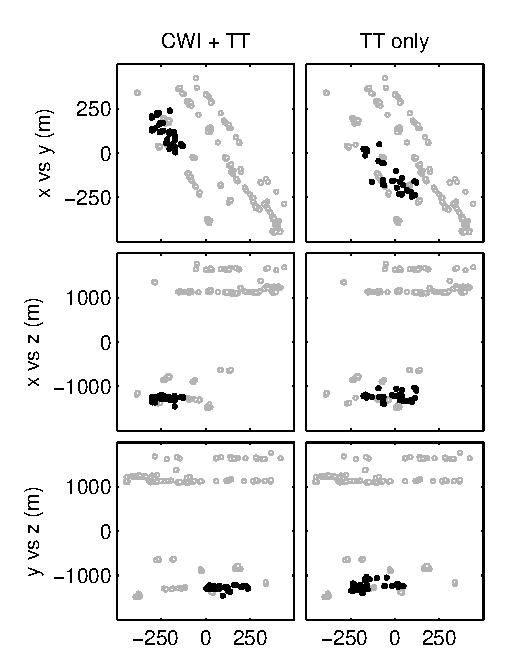
\includegraphics{diags/CalaverasLoc6_hypoDD_SVD.eps}
\caption{Example 8 - Mimicking the deployment of a temporary network
by ignoring data from all but station CCO for 50\% (or 34) of the
events. Relative locations are shown for the combined CWI and travel
time inversion (left) and the inversion with travel times only
(right) Only by combining the data is it possible to locate all 68
events. Furthermore, combining the data leads to a solution more
consistent with Figure \ref{fig-69Calaverasevents_eg1}. }
\label{fig-68Calaverasevents_ttsubsetandcoda1}
\end{figure}
%%=========================================================================



\section{Discussion and Conclusions}

Coda wave interferometry is an emerging technique for constraining
earthquake location. The technique relies on the interference
between coda waves of closely located events and is hence useful for
studying earthquake clusters and/or aftershock sequences. Coda wave
constraints are independent of travel times and can be used in
isolation or combination with early onset body waves. The strength
of coda is that it is possible to constrain earthquake location from
a single station, an outcome demonstrated most clearly by Figures
\ref{fig-CWIreducesstats} and
\ref{fig-68Calaverasevents_ttsubsetandcoda1}.

Coda wave interferometry offers a new technique for understanding
earthquakes in intraplate areas with sparse networks and poor
azimuthal coverage. In particular, the ability to combine coda wave
constraints with travel times makes it possible to link well
constrained events from a temporary deployment with those recorded
outside the deployment period. All that is required to achieve this
is at least one network station which has recorded sufficient events
from both periods. CWI facilitates the location of poorly recorded
events to an accuracy approaching those recorded during the
temporary deployment and therefore opens new avenues for imaging
intraplate fault structures and improved our understanding of
intraplate seismicity and earthquake hazard.

Another potential application of CWI is in the area of hydraulic
fracturing such as hot rock geothermal projects and/or petroleum
reservoir engineering. Monitoring pumping induced micro earthquakes
is a key step in understanding the migration of fluids in such
reservoirs. There is a trade-off in the ability of surface deployed
networks to locate events which are small and/or deep. Downhole
seismic monitoring is likely to play increasingly important roles in
deep reservoir projects. CWI creates new possibilities to monitor
pumping induced micro earthquakes from fewer boreholes and hence
dramatically reduce the costs of reservoir monitoring at large
depths. It may also be possible to utilize coda for understanding
hazard in tunneled mining operations where the location of deep
tunnels prohibits azimuthal coverage of induced events.

\section{Data and Resources}
We thank the Northern California Earthquake Data Center (NCEDC) for
providing the Calaveras data and the Northern California Seismic
Network (NCSN), U.S. Geological Survey, Menlo Park and Berkeley
Seismological Laboratory, University of California, Berkeley for
contributing it to the NCEDC. The waveforms can be downloaded from
http://www.ncedc.org/ncedc/access.html. We also acknowledge Felix
Waldhauser and William Ellsworth, the authors of the openly
available Double Difference location algorithm, hypoDD which can be
downloaded from http://www.ldeo.columbia.edu/~felixw/hypoDD.html.


\begin{acknowledgments}
Geoscience Australia, the Research School of Earth Sciences at The
Australian National University, and the Center for Wave Phenomena at
the Colorado School of Mines, are acknowledged for supporting this
research. The paper is published with permission of the CEO
Geoscience Australia. Work was conducted as part of an Australian
Research Council Discovery Project (DP0665111).  This paper has
benefited significantly from reviews by ......... at Geoscience
Australia.
\end{acknowledgments}


\bibliography{../refs/drrefs}




\appendix

\section{The noisy likelihood}
\label{sec-Appendix-noisylikelihood}

The noisy likelihood
$P(\widetilde{\delta}_{CWIN}|\widetilde{\delta}_t)$ used in equation
(\ref{eq:-bayesian-noisyform}) is given by
\begin{equation}
\begin{array}{l}
\label{eq-likelihood-int}
P(\widetilde{\delta}_{CWIN}|\widetilde{\delta}_t)  =
A(\widetilde{\delta}_t) C(\bar{\mu}_N, \bar{\sigma}_N)  \\
\hspace{3em} \times \int_0^\infty
B(\widetilde{\delta}_t,\widetilde{\delta}_{CWI})
D(\widetilde{\delta}_{CWI},\bar{\sigma}_N,\bar{\mu}_N )
d\widetilde{\delta}_{CWI}
\end{array}
\end{equation}
where $\widetilde{\delta}_{CWI}$ is an estimate of CWI separation in the absence
of noise,
\begin{equation}
\label{eq:Adefn}
A(\widetilde{\delta}_t) = \frac{1}{(1-\Phi_{\mu_1,\sigma_1}(0))\sigma_1\sqrt{2\pi} },
\end{equation}
\begin{equation}
B(\widetilde{\delta}_t,\widetilde{\delta}_{CWI})=e^{  \frac{-(\widetilde{\delta}_{CWI}-\mu_1)^2}{2\sigma_1^2} },
\end{equation}
\begin{equation}
\label{eq:Cdefn}
C(\bar{\mu}_N, \bar{\sigma}_N) =  \frac{1}{(1-\Phi_{\bar{\mu}_N,\bar{\sigma}_N}(0))\sigma_N\sqrt{2\pi}},
\end{equation}
\begin{equation}
D(\widetilde{\delta}_{CWI},\bar{\sigma}_N,\bar{\mu}_N )=e^{  \frac{-(\widetilde{\delta}_{CWI}-\bar{\mu}_N)^2}{2 \bar{\sigma}_N ^2} }
\end{equation}
and $\Phi_{\mu,\sigma}(x)$ is the cumulative Gaussian distribution function
\begin{equation}
\label{eq-cummulative-Gaussian}
\Phi_{\mu,\sigma}(x) = \frac{1}{\sigma \sqrt{2 \pi}}
\int_{-\infty}^x e^{  \frac{-(s-\mu)^2}{2\sigma^2}  } ds
\end{equation}
\citep{dr_Robinson11a}. The parameters $\mu_1$ and $\sigma_1$ used
in equation (\ref{eq:Adefn}) are defined by the expressions
\begin{equation}
\label{eq:mu1}
\mu_1(\widetilde{\delta}_t) = a_1\frac{a_2 \widetilde{\delta}_t^{a_4}+a_3
\widetilde{\delta}_t^{a_5}}{a_2 \widetilde{\delta}_t^{a_4}+a_3 \widetilde{\delta_t}^{a_5}+1}
\end{equation}
and
\begin{equation}
\label{eq:sigma1}
\sigma_1(\widetilde{\delta}_t) = c + a_1\frac{a_2 \widetilde{\delta}_t^{a_4}+
a_3 \widetilde{\delta}_t^{a_5}}{a_2 \widetilde{\delta}_t^{a_4}+a_3 \widetilde{\delta}_t^{a_5}+1}
\end{equation}
with coefficients $a_1$ to $a_5$ and $c$ defined in Table
\ref{tab-const4-mu1-sigma1}. The parameters $\bar{\mu}_N$ and
$\bar{\sigma}_N$ used in equation (\ref{eq:Cdefn}) are obtained by
finding the values which minimize the difference in a least squares
sense between the noisy CWI estimates $\widetilde{\delta}_{CWIN}$
computed from the waveforms and the positively bounded Gaussian
density function
\begin{equation}
\label{eq-likelihood-noisydata-pdf-orig}
\begin{array}{l}
P(\widetilde{\delta}_{CWIN}|\widetilde{\delta}_t,\widetilde{\delta}_{CWI}) \\
\hspace{5em} = \frac{1}{\left(1-\Phi_{\bar{\mu}_N,\bar{\sigma}_N}(0)\right)\bar{\sigma}_N\sqrt{2\pi}}
e^{  \frac{-(\widetilde{\delta}_{CWIN}-\bar{\mu}_N)^2}{2\bar{\sigma}_N^2}  }
\end{array}
\end{equation}
with $\widetilde{\delta}_{CWIN} \geq 0$.


\begin{table}
\caption{Coefficients for equations. (\ref{eq:mu1}) and
(\ref{eq:sigma1}).} \label{tab-const4-mu1-sigma1}
\begin{tabular}{|c|c|}
\hline
$\mu_1(\widetilde{\delta}_t)$ & $\sigma_1(\widetilde{\delta}_t)$ \\
\hline
$a1 = 0.4661$ & $a1 = 0.1441$\\
$a2 = 48.9697$ & $a2 = 101.0376$\\
$a3 = 2.4693$ & $a3 = 120.3864$\\
$a4 = 4.2467$ & $a4 = 2.8430$\\
$a5 = 1.1619$ & $a5 = 6.0823$ \\
     & $c = 0.017$ \\
\hline
\end{tabular}
\end{table}


\section{Derivatives}
\label{sec-Appendix-derivatives_ofL}

The derivatives of $L(\mathbf{e}_1,\mathbf{e}_2,...,\mathbf{e}_N)$
\begin{equation}
\frac{\partial L}{\partial \hat{x}_1},
\frac{\partial L}{\partial \hat{y}_1},
 \frac{\partial L}{\partial \hat{z}_1},
\frac{\partial L}{\partial \hat{x}_2},
\frac{\partial L}{\partial \hat{y}_2},
\frac{\partial L}{\partial \hat{z}_2},
...,
\frac{\partial L}{\partial \hat{x}_N},
\frac{\partial L}{\partial \hat{y}_N},
\frac{\partial L}{\partial \hat{z}_N}
\end{equation}
are required by the Polak-Ribiere algorithm. These are used to guide
the optimization procedure towards the values of
$(\mathbf{e}_1,\mathbf{e}_2,...,\mathbf{e}_N)$ which minimize $L$.

The equations for the derivatives are convoluted so we build them
gradually. We start with an expression for $\delta_t$, the
wavelength normalized separation between two events $\mathbf{e}_p=
(\hat{x}_p,\hat{y}_p,\hat{z}_p)$ and $\mathbf{e}_q =
(\hat{x}_q,\hat{y}_q,\hat{z}_q)$
\begin{equation}
\label{eq:deltat4chapt6deriv}
\delta_t = \frac{f_{dom}}{v_s}\sqrt{(\hat{x}_p-\hat{x}_q)^2 + (\hat{y}_p-\hat{y}_q)^2 +  (\hat{z}_p-\hat{z}_q)^2},
\end{equation}
where $f_{dom}$ is the dominant frequency of the waveforms and $v_s$ is the velocity between the events. Expression
\ref{eq:deltat4chapt6deriv} has derivatives
\begin{equation}
\label{eq-partial-xyz1}
\begin{array}{l}
\frac{\partial \widetilde{\delta}_t}{\partial \hat{x}_p} = \frac{f_{dom}^2 (\hat{x}_p-\hat{x}_q)}{v_s^2 \widetilde{\delta}_t},
\frac{\partial \widetilde{\delta}_t}{\partial \hat{y}_p} = \frac{f_{dom}^2 (\hat{y}_p-\hat{y}_q)}{v_s^2 \widetilde{\delta}_t}, \\
\frac{\partial \widetilde{\delta}_t}{\partial \hat{z}_p} = \frac{f_{dom}^2 (\hat{z}_p-\hat{z}_q)}{v_s^2 \widetilde{\delta}_t},
\frac{\partial \widetilde{\delta}_t}{\partial \hat{x}_q} = \frac{f_{dom}^2 (\hat{x}_q-\hat{x}_p)}{v_s^2 \widetilde{\delta}_t}, \\
\frac{\partial \widetilde{\delta}_t}{\partial \hat{y}_q} = \frac{f_{dom}^2 (\hat{y}_q-\hat{y}_p)}{v_s^2 \widetilde{\delta}_t},
\frac{\partial \widetilde{\delta}_t}{\partial \hat{z}_q} = \frac{f_{dom}^2 (\hat{z}_q-\hat{z}_p)}{v_s^2 \widetilde{\delta}_t}.
\end{array}
\end{equation}
For brevity we focus the following derivation in terms of $\hat{x}_p$. The remaining terms for $\mathbf{e}_p$
(i.e. $\hat{y}_p$ and $\hat{z}_p$) can be computed
by following the same procedure. The derivatives for $\mathbf{e}_q$ can be attained by exploiting the symmetry
\begin{equation}
\label{eq:ep2eq-deriv-symmetry}
\frac{\partial \widetilde{\delta}_t}{\partial \hat{x}_q} = - \frac{\partial \widetilde{\delta}_t}{\partial \hat{x}_p}.
\end{equation}

The chain rule gives
\begin{equation}
\frac{\partial \mu_1}{\partial \hat{x}_p} = \frac{\partial \mu_1}{\partial \widetilde{\delta}_t} \frac{\partial \widetilde{\delta}_t}{\partial \hat{x}_p}
\end{equation}
where differentiating equation (\ref{eq:mu1}) gives
\begin{equation}
\label{eq-dmu1-by-dx1}
\frac{\partial \mu_1}{\partial \widetilde{\delta}_t} = a_1 \frac{a_2 a_4 \widetilde{\delta}_t^{a_4-1} +a_3 a_5 \widetilde{\delta}_t^{a_5-1}}
{\left(a_2 \widetilde{\delta}_t^{a_4} +a_3 \widetilde{\delta}_t^{a_5} +1 \right)^2}.
\end{equation}
Similarly, we have
\begin{equation}
\frac{\partial \sigma_1}{\partial \hat{x}_p} = \frac{\partial \sigma_1}{\partial \widetilde{\delta}_t} \frac{\partial \widetilde{\delta}_t}
{\partial \hat{x}_p}
\end{equation}
where $\frac{\partial \sigma_1}{\partial \widetilde{\delta}_t}$ has the identical form as \ref{eq-dmu1-by-dx1} with different constants
$a_1,a_2,...,a_5$ (see table \ref{tab-const4-mu1-sigma1}).

The cumulative Gaussian distribution function \ref{eq-cummulative-Gaussian} is
\begin{equation}
\Phi_{\mu_1,\sigma_1}(0) = \frac{1}{\sigma_1 \sqrt{2 \pi}}
\int_{-\infty}^0 e^{  \frac{-(s-\mu_1)^2}{2\sigma_1^2}  } ds
\end{equation}
which has derivative
\begin{equation}
\frac{\partial \Phi_{\mu_1,\sigma_1}(0)}{\partial \hat{x}_p} =
\frac{ \sigma_1 \int_{-\infty}^0 \frac{\partial g}{\partial \hat{x}_p} e^g ds -
\frac{\partial \sigma_1}{\partial \hat{x}_p} \int_{-\infty}^0 e^g ds}
{\sigma_1^2 \sqrt{2 \pi}}
\end{equation}
where
\begin{equation}
g = \frac{-(s-\mu_1)^2}{2 \sigma_1^2}
\end{equation}
and
\begin{equation}
\frac{\partial g}{\partial \hat{x}_p} = \frac{4 \sigma_1^2 (s-\mu_1) \frac{\partial \mu_1}{\partial \hat{x}_p}
+ 4\sigma_1 \frac{\partial \sigma_1}{\partial \hat{x}_p}(s-\mu_1)^2}
{4 \sigma_1^4}.
\end{equation}

Now, we have all the pieces to compute the derivatives of $A=A(\delta_t)$ and $B = B(\delta_t,\delta_{CWI})$ as follows
\begin{equation}
\frac{\partial A} {\partial \hat{x}_p} =
-\frac{ -\frac{\partial  \Phi_{\mu_1,\sigma_1}(0)}{\partial \hat{x}_p} \sigma_1 +
 \left(1- \Phi_{\mu_1,\sigma_1}(0) \right) \frac{\partial \sigma_1}{\partial \hat{x}_p}}
{\left(1- \Phi_{\mu_1,\sigma_1}(0) \right)^2 \sigma_1^2 \sqrt{2 \pi}}
\end{equation}
and
\begin{equation}
\frac{\partial B} {\partial \hat{x}_p} = e^h \frac{\partial h}{\partial \hat{x}_p}
\end{equation}
where
\begin{equation}
h =  \frac{-(\delta_{CWI}-\mu_1)^2}{2 \sigma_1^2}
\end{equation}
and
\begin{equation}
\frac{\partial h}{\partial \hat{x}_p} = \frac{
4 \sigma_1^2 (\delta_{CWI}-\mu_1) \frac{\partial \mu_1}{\partial \hat{x}_p}
+ 4(\delta_{CWI}-\mu_1)^2 \sigma_1 \frac{\partial \sigma_1}{\partial \hat{x}_p} }
{4 \sigma_1^4}.
\end{equation}
Finally, we can differentiate the likelihood for an individual event pair
\begin{equation}
\begin{array}{l}
\frac{\partial P(\delta_{CWIN}|\widetilde{\delta}_t)} {\partial \hat{x}_p}  =
\frac{\partial A(\widetilde{\delta}_t)}{\partial \hat{x}_p} C(\bar{\mu}_N, \bar{\sigma}_N) \\
\hspace{2em} \times \int_0^\infty B(\widetilde{\delta}_t,\widetilde{\delta}_{CWI})
D(\widetilde{\delta}_{CWI},\bar{\sigma}_N,\bar{\mu}_N )
d\widetilde{\delta}_{CWI} \\
\hspace{2em} + A(\widetilde{\delta}_t) C(\bar{\mu}_N, \bar{\sigma}_N) \\
\hspace{2em} \times \int_0^\infty
\frac{\partial B(\widetilde{\delta}_t,\widetilde{\delta}_{CWI})} {\partial \hat{x}_p}
D(\widetilde{\delta}_{CWI},\bar{\sigma}_N,\bar{\mu}_N )
d\widetilde{\delta}_{CWI}
\end{array}
\end{equation}
and for the logarithm we have
\begin{equation}
\frac{ \partial \ln \left[ P(\delta_{CWIN}|\delta_t) \right] } {\partial \hat{x}_p}
= \frac{1}{P(\delta_{CWIN}|\delta_t)} \frac{\partial P(\delta_{CWIN}|\delta_t)}{\partial \hat{x}_p}.
\end{equation}


Thus, it follows that the derivative of $L$ with respect to $\hat{x}_p$ is given by
%\begin{equation}
%\label{eq-derivative-Lstar-cwionly22}
%\frac{\partial L(E_1, E_2, ..., E_n)}{\partial \hat{x}_p} =
%- \sum_{i=p+1}^{N} \frac{ \partial \ln \left[P(\delta_{CWIN}|E_p,E_i)\right]}{\partial \hat{x}_p}
%+ \sum_{j=1}^{p-1} \frac{ \partial \ln \left[P(\delta_{CWIN}|E_j,E_p)\right]}{\partial \hat{x}_p}
%\end{equation}
\begin{equation}
\label{eq-derivative-Lstar-cwionly}
\begin{array}{ll}
\frac{\partial L(E_1, E_2, ..., E_n)}{\partial \hat{x}_p} = &
- \sum_{i=p+1}^{N} \frac{ \partial \ln \left[P(\delta_{CWIN}|E_p,E_i)\right]}{\partial \hat{x}_p} \\
 & + \sum_{j=1}^{p-1} \frac{ \partial \ln \left[P(\delta_{CWIN}|E_j,E_p)\right]}{\partial \hat{x}_p}
\end{array}
\end{equation}
%
%\iftwocol{\begin{eqnarray} \frac{\partial L(E_1, E_2, ..., E_n)}{\partial \hat{x}_p} &  = &\\
%- \sum_{i=p+1}^{N} \frac{ \partial \ln \left[P(\delta_{CWIN}|E_p,E_i)\right]}{\partial \hat{x}_p} \\
%+ \sum_{j=1}^{p-1} \frac{ \partial \ln \left[P(\delta_{CWIN}|E_j,E_p)\right]}{\partial \hat{x}_p}
%\end{eqnarray}}
%{\frac{\partial L(E_1, E_2, ..., E_n)}{\partial \hat{x}_p} =
%- \sum_{i=p+1}^{N} \frac{ \partial \ln \left[P(\delta_{CWIN}|E_p,E_i)\right]}{\partial \hat{x}_p}
%+ \sum_{j=1}^{p-1} \frac{ \partial \ln \left[P(\delta_{CWIN}|E_j,E_p)\right]}{\partial \hat{x}_p}}
%\end{equation}
for a uniform prior. The change of sign in the middle (i.e. to
addition) accounts for the change in order of the events under the
conditional. Its inclusion here assumes the correct use of $\partial
\widetilde{\delta}_t / \partial \hat{x}_p$ or $\partial
\widetilde{\delta}_t / \partial \hat{x}_q$ when evaluating the left
and right hand terms of the summation. The derivatives shown in this
section appear complicated but are in practice trivial to compute
numerically. Confidence in their accuracy is enhanced by
demonstrating that the optimization procedure converges to the
correct solution for a number of synthetic problems in 2 and 3
dimensions.


\clearpage








%\bsp % ``This paper has been produced using the Blackwell
     %   Publishing GJI \LaTeXe\ class file.''

\label{lastpage}


\end{document}
